\part{Experiment}\label{part:experiment}
\chapter{Quantum network apparatus design}\label{ch:nodes}
% the hierarchy is 
% chapter,section,subsection,etc

An outstanding technical challenge for cold atom technologies, including but not limited to quantum networks and processors, is reducing the footprint of these often space-consuming apparatuses. Building more compact cold atom science platforms is of both academic and potential commercial interest, and our implementation is one of several demonstrated approaches to date (?? CITE some of the on-chip stuff, think Aidan Arnold, also CAL. See what has been shared in Kats slack). The approach we present here makes use of relatively small bulk optics which are pre-aligned and placed in the UHV chamber and connected to by fiber optic feedthroughs, making for a plug-and-play quantum testbed. The design and construction procedure for our apparatus is outlined in the remainder of this chapter.

\section{Quantum Network Node Design}
\subsection{On-chip optical architecture}

Cold atom experiments often require on the order of ten different laser beams directed into a vacuum chamber, each having optics to tune the direction, beam size, polarization; and optics for photon collection for state readout. In this work, we present a compact architecture in which light is brought into and out of the vacuum system by optical fiber feedthroughs and the light is sent to and collected from the atoms using in-vacuum optics. 
%A schematic of the apparatus is shown in Fig. \ref{fig:network_node_apparatus_schematic}.

% \begin{figure}[!ht]
%     \centering
%     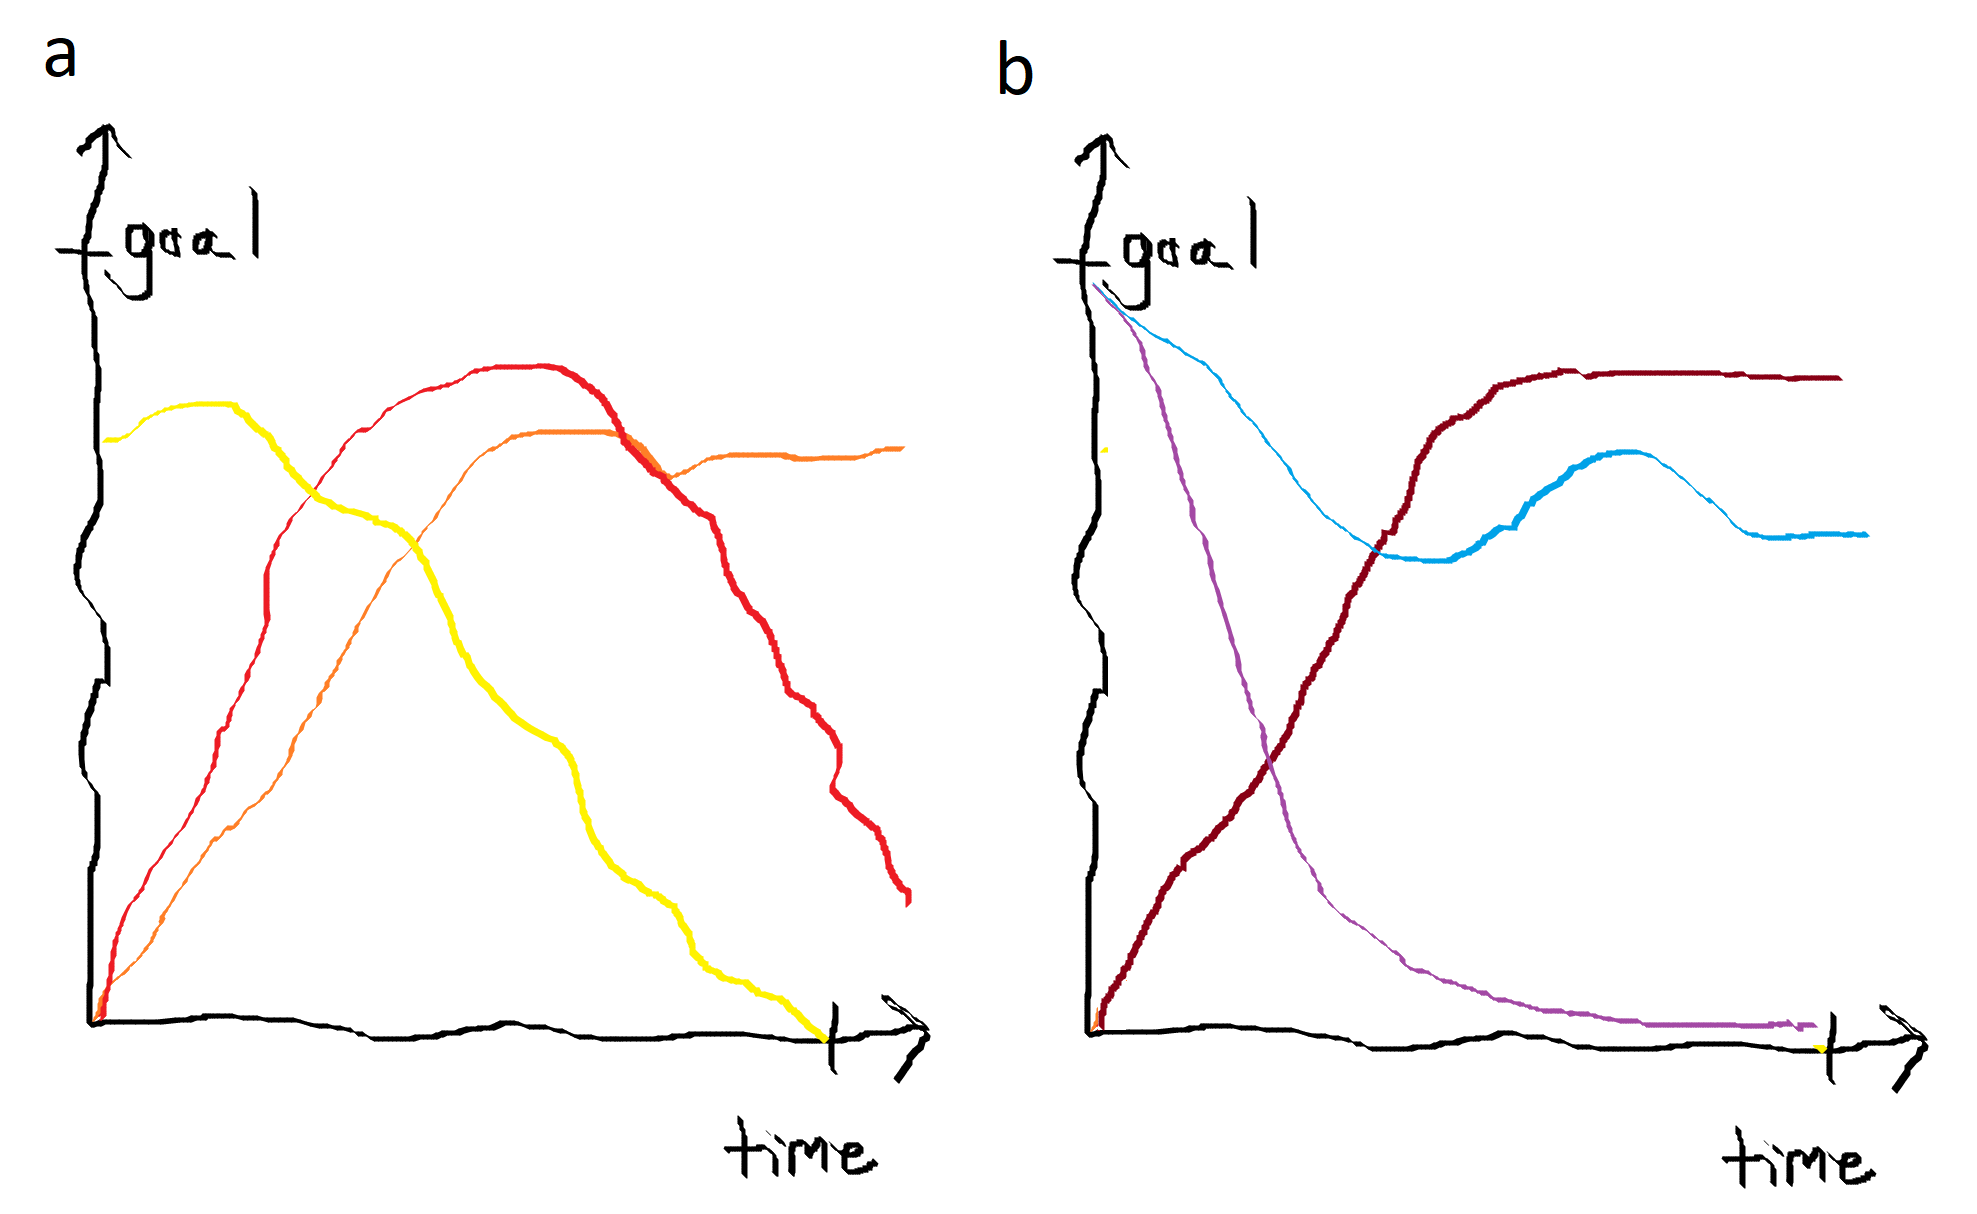
\includegraphics[width=0.45\textwidth]{Images/fig_coming_soon.png}
%     \caption{A schematic of the apparatus}
%     \label{fig:network_node_apparatus_schematic}
% \end{figure}

The in-vacuum optics are installed on a custom substrate  machined out of Macor. Macor was chosen for its low thermal expansion, mechanical strength, and ability to be machined easily using common tools such as a Dremel. This last point proved important, as it provided some insurance against some unforeseen mechanical conflicts during optical assembly. The Macor substrate, henceforth referred to as either bridge or chip, interchangeably, was designed to accommodate different optical modules consisting of bulk optics which map the light from fiber to free space beams and set the polarization. The layout of the optics for the first version of the quantum network node is shown schematically in Fig. (\ref{fig:optical_chip_design}) Each optical module, described in detail in the following sections, was individually assembled then aligned and glued to the bridge using low-outgassing epoxy. 

\begin{figure}[!ht]
    \centering
    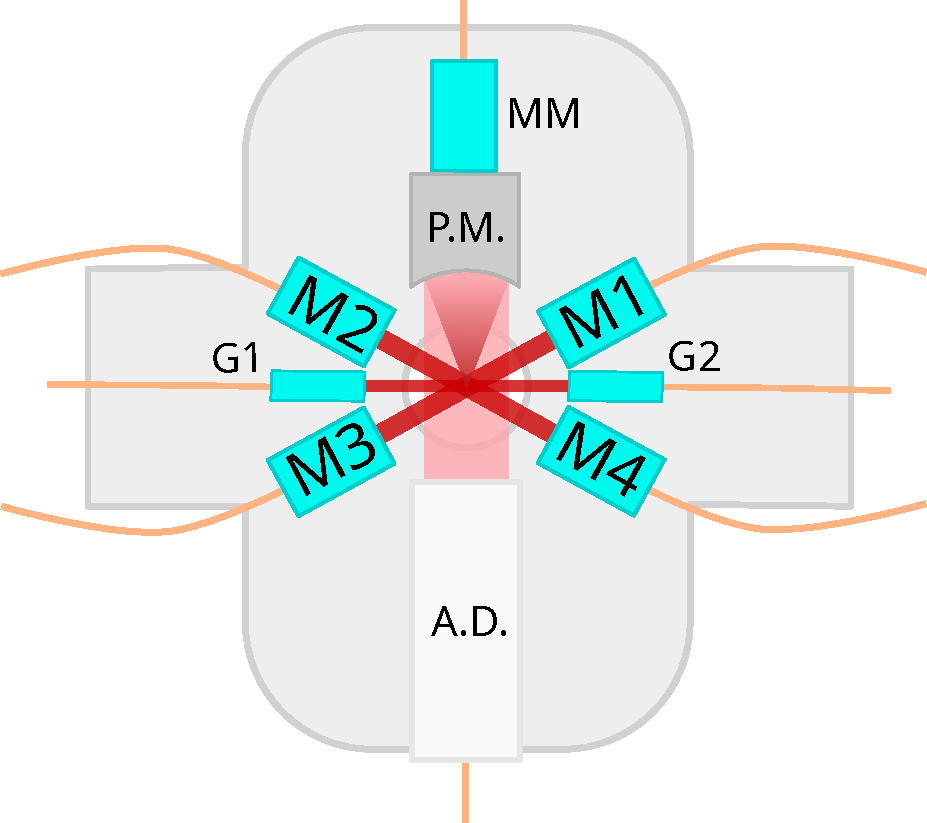
\includegraphics[width=0.45\textwidth]{Images/optical_chip_schematic.pdf}
    \caption{A simplified illustration of the layout of optical modules on the Macor bridge for the first version of the quantum network node. The modules M1-M4 (MOT 1 - MOT 4 in the text) produce the four MOT arms in a plane parallel to the bridge, G1 and G2 (GRIN 1 and GRIN 2 in the text) produce beams for optical pumping and excitation for Bell state preparation, P.M. is the parabolic mirror, and A.D. houses an achromatic doublet. In reality, A.D. and P.M. are a single optical module, but are shown separately here for clarity. MM couples light which passes through a central hole in the parabolic mirror and then a polarizer into a multimode fiber. Each module is interfaced with a polyamide coating optical fiber (orange lines), which allows coupling  light from outside the vacuum system. See Sec. \ref{sec:science_optics} for more details on the optical modules.}
    \label{fig:optical_chip_design}
\end{figure}

\subsection{Vacuum system design}
%An illustrative cross-section of the quantum network node UHV system is shown in Fig. \ref{fig:vacuum_cross_section}. 

The vacuum system consists of a custom science chamber in which the optics live, a valve and bellows to store an atomic ampule, two ion pumps (Edwards 10S TiTan), and valves for pumping down the system. A SOLIDWORKS model is shown in Fig. \ref{fig:vacuum_chamber_model}

\begin{figure}
    \centering
    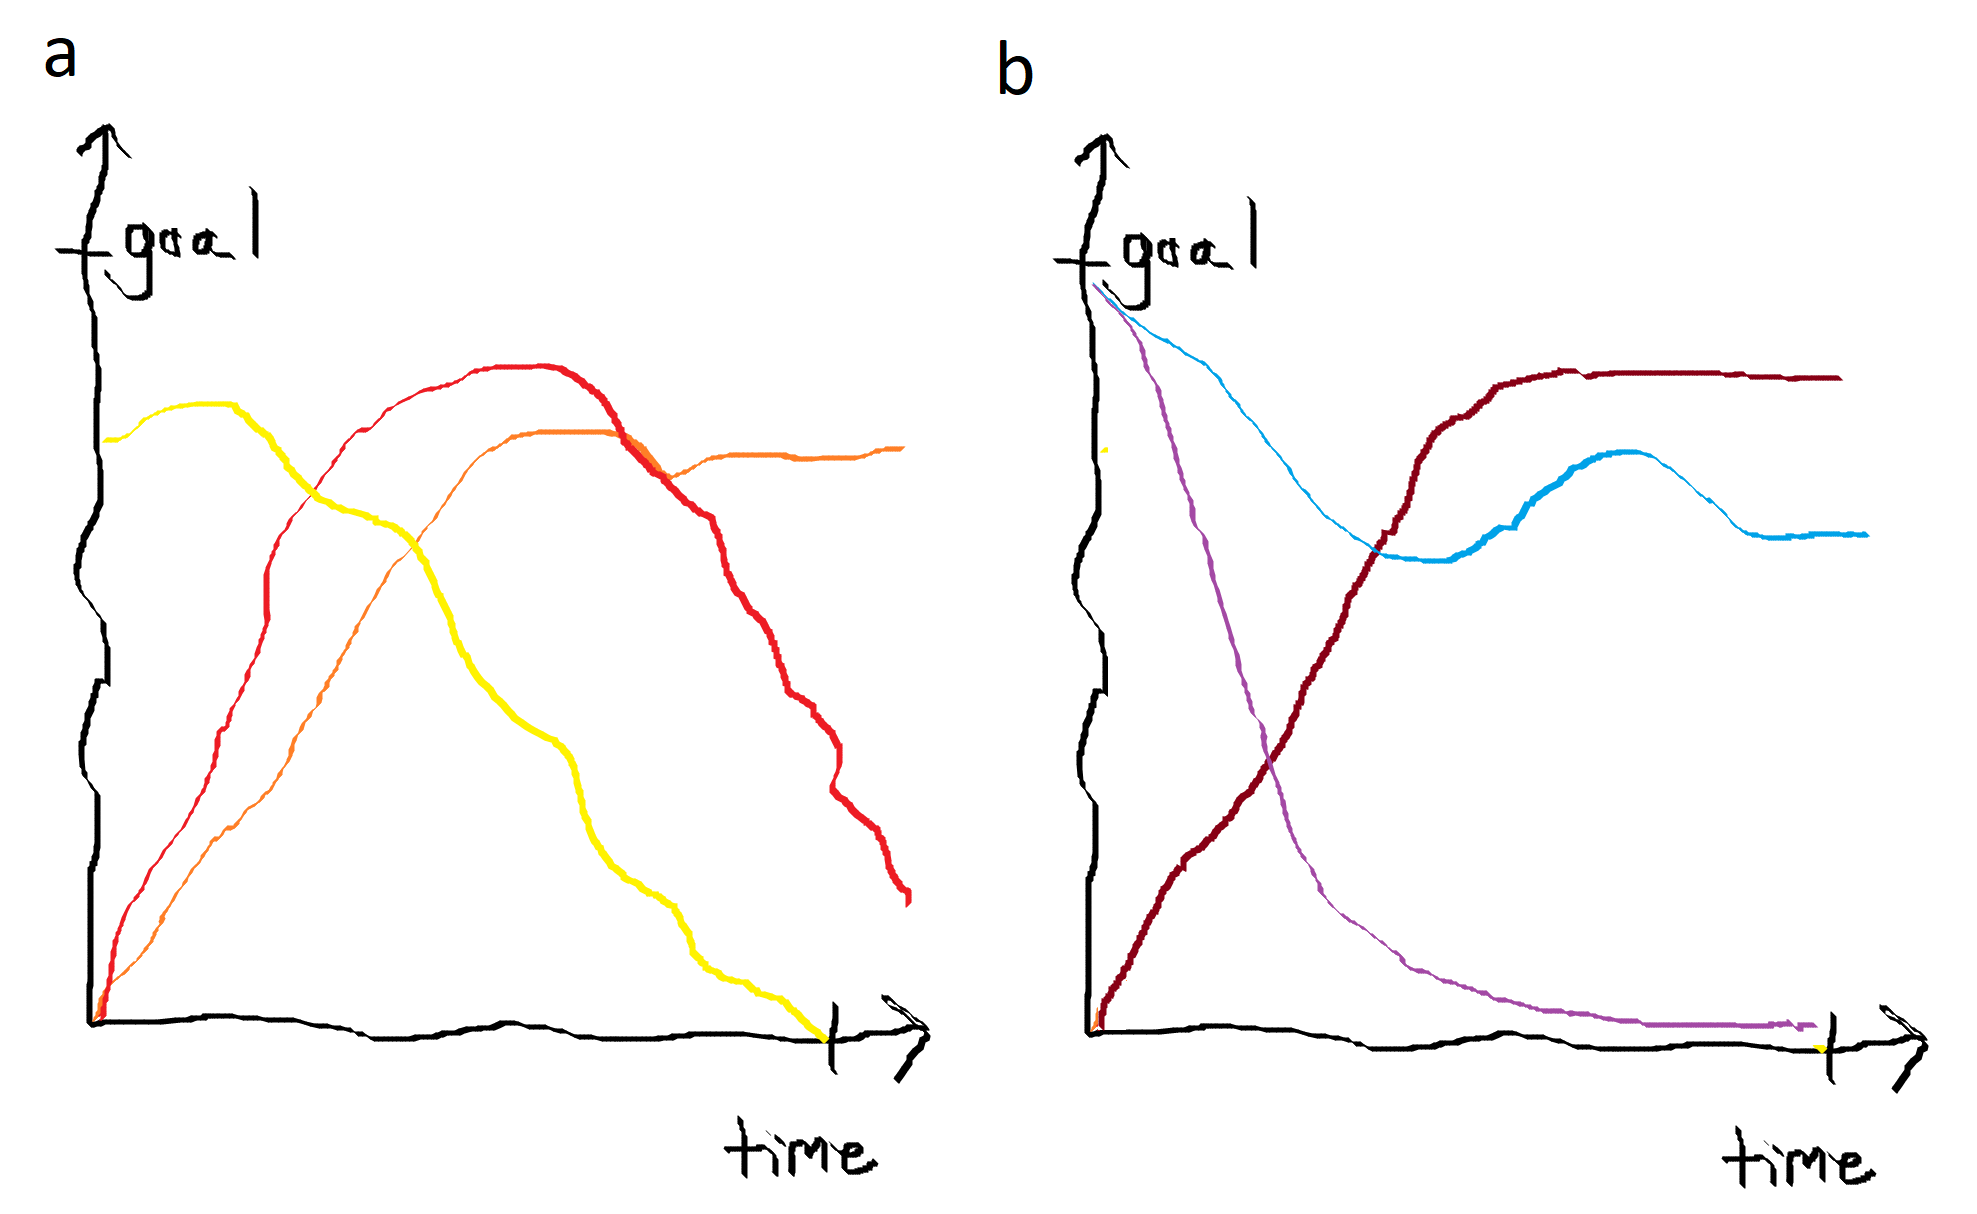
\includegraphics{Images/fig_coming_soon.png}
    \caption{Caption coming soon}
    \label{fig:vacuum_chamber_model}
\end{figure}

The custom stainless steel chamber (MDC Precision) which houses the optical chip is modeled in the fashion of a pair of 6" Conflat flanges, furnished with fused silica view ports on each side for external optical access. The view ports are AR coated on both sides for 400-1100 nm and the thickness of each was chosen so as to cancel optical aberrations when used with existing custom objective lenses (JenOptik) used in our group. The Macor chip holding the optics mounts into the chamber with the help of two Kimball Physics Groove Grabbers (6", Reverse) which mount to the inner wall of the lower half of the science chamber. The chip is situated such that the plane defined by the axes of the optical beams on the chip, and hence the region where an atom will be trapped, is equidistant from each window. See the mechanical drawing in Appendix \ref{ch:mech_drawings} for the full dimensions of the science chamber.

\begin{figure}
    \centering
    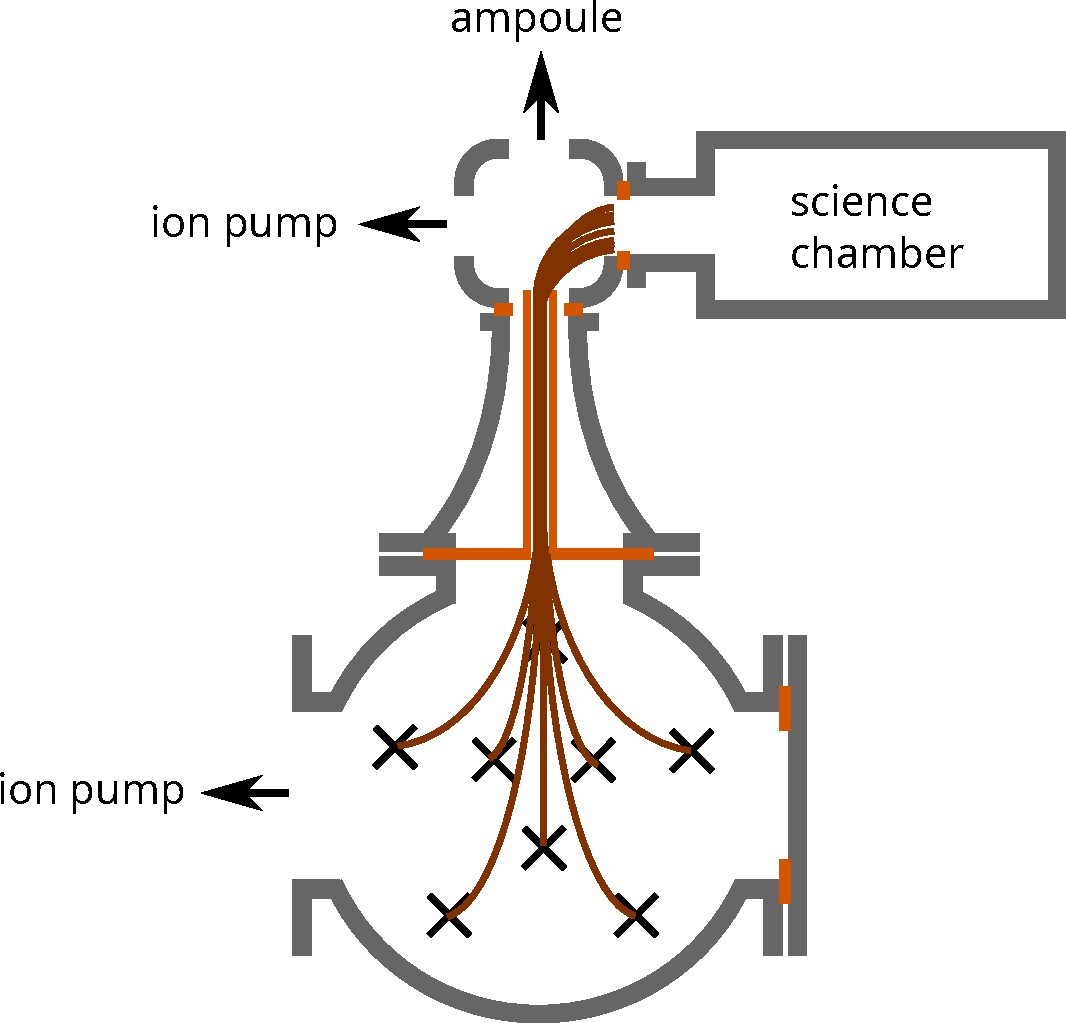
\includegraphics[width=0.5\textwidth]{Images/differential_pumping.pdf}
    \caption{A cross-section illustration showing the copper pinch off tube used as a differential pumping tube between the upper and lower vacuum chamber regions. The 8 fibers coming through the drilled Teflon plugged SwageLock feedthroughs (each feedthrough marked as a black X) go up through the copper tube and into the science region.}
    \label{fig:differential_pumping}
\end{figure}

The vacuum system is divided into two sections, upper and lower, separated by a differential pumping region. This is done in order to shield the science region from small leaks which may be present due to the eight fiber feedthroughs in use. In the section joining the upper and lower chambers, a copper pinch-off tube, cut to a length of 7 cm and with tube inner diameter 6.35 mm, was used in lieu of a standard Conflat copper gasket (see Fig. \ref{fig:differential_pumping}). Additionally, the middle section of the tube was pinched down to approximately a slit of 1 mm width to further reduce the flow conductivity between the two regions. An upper bound for the conductivity of the pipe can be estimated by ignoring the pinch and using the Knudsen flow conductivity in the molecular flow regime (valid for our UHV pressure level),
\begin{equation}
     C = 12.1\frac{d^3}{l}
\end{equation}
for a pipe of diameter $d$ and length $l$, where $l \geq 10d$ \cite{Marquardt1999}. This gives a conductivity of 0.44 L/s between the two chambers, which is lower than the upper ion pump's pumping speed, 10 L/s, by a factor of about 22. The actual conductivity is lower due to the pinch, and the conductivity between the science region and lower chamber is lower still due to the right angle between the science chamber and differential pumping path. In practice, we observed an order of magnitude difference ($P_{\textrm{upper}}=4\cdot10^{-10}$ Torr, compared to $P_{\textrm{lower}}=2\cdot10^{-9}$ Torr) between the two chambers following the vacuum bakeout and prior to opening the valve to release Rb vapor.

\section{UHV science optics}\label{sec:science_optics}

Optics for preparing laser cooling beams, state preparation beams, optical dipole trap, and photon collection are installed in our UHV system. Each beam is prepared by an optical module consisting of a fiber connected to a ferrule installed in a tube containing other optics, including lenses, polarizers, and waveplates, depending on the purpose of the particular module. The components of each module are aligned and glued together using UV-curable UHV-safe epoxy (Optocast 3410 Gen2). The Macor bridge was designed with grooves to pre-align each module, however, some manual alignment of position was required, in addition to alignment of polarization for some of the beams. Active alignment of optics in vacuum, e.g. by piezo control, was foregone in favor of simplifying the apparatus design. In the following sections, the construction of each type of optical module and the subsequent co-alignment of all of the beams is described. 

In the first version of our quantum network node design, the optics in UHV consisted of modules for creating four of six laser cooling beams, two optical pumping/excitation beams, and a simultaneous dipole trap and photon collection path based on a high-NA on-axis parabolic mirror. A complete ``ingredient list" of the parts required to build this version of the network is given in Appendix \ref{ch:ingredients}.

\subsection{Clean room assembly environments}

All of the assembly of the UHV optical components took place inside of two table-top enclosures which mimic a clean room environment. Each enclosure has a HEPA-filtered fan to provide positive pressure from clean air over the optics and tools inside. One of the enclosures or ``clean boxes" was a commercially available solution by Sentry Air Systems (model SS-218-PCR), while the other was custom constructed from transparent acrylic sheets but used the same Sentry Air Systems air purifier (model SS-200-MS). The custom box measured roughly 1 m wide by 0.5 m deep and 0.5 meter tall, about twice the width of the commercial box. Particulate matter levels were tracked in the custom box using a Temtop PMD 331 particle counter, which counts particles of various sizes down to 2.5 $\mu$m. Typical particle counts observed were consistent with a class ISO 4 clean room.

\subsection{MOT and state preparation optics}
Below we discuss the design and construction of optical modules consisting of relatively small bulk optics which set the beam size and polarization of the light for manipulating the atomic states of interest. The assembly of these modules was done mostly by hand with the aid of some custom holders which we 3D printed, a fiber holder (Thorlabs HFF001), and assorted 3-axis translation stages. The procedure is described in what follows. For the first network node, each of these modules was constructed with care by Akbar Safari.

\subsubsection{MOT optics}

The in-vacuum optics for delivering the cooling light, MOT repumper, and excitation repumper consisted of four optical modules which we will refer to as ``MOT tubes" going forward. The MOT tubes are labeled $M1-M4$ in the schematic in Fig. \ref{fig:optical_chip_design}. These four modules create beams in a plane parallel to that of the Macor substrate, whereas the other two MOT beams are delivered by free space optics mounted outside of the chamber. Each MOT tube, with a form factor of $\sim1$ cm$^3$, is used to terminate a PM fiber and replaces the chain of larger bulk optics that would typically be used for creating MOT beams. Specifically, each MOT tube consists of a fiber ferrule, collimating lens ($f=5$ mm, Edmund Optics $\#$48-709), polarizer (Skight Optics, AR coated for 780 nm), and quarter waveplate (Skight Optics, zero-order for 780 nm, AR coated). All of these components are safe for use in UHV. In cases where the manufacturer was unable to guarantee this, we tested components in a small UHV chamber to ensure outgassing (e.g. from optical epoxy or coatings) did not inhibit reaching vacuum at the level of $10^{-10}$ Torr. The optical fibers used (Fibercore HB800P/001), including those used for the other optical modules discussed later in this work, are polyimide coated, which is safe for use in UHV and makes the fiber more resistant to breaking compared to bare fiber. The components for each MOT tube are housed in a 7mm outer diameter glass tube which can be co-aligned to the other optics on the Macor substrate. Each glass tube has two holes drilled in specific locations to allow air to be pumped out from the regions between the polarizer and lens and between lens and the fiber.

For each MOT tube, a PM fiber of approximately 2 m in length was used, where one end was connectorized with an APC connector and the other end was cleaved. We initially used a bare fiber adapter to couple into the fiber, but found this to be mechanically unstable. The connector facilitated more stable coupling of light into the fiber during the alignment procedure. The cleaved end of the fiber was inserted and glued into a fiber ferrule which in turn was inserted and glued into a Macor sleeve, which held the 1.8 mm diameter ferrule in the 5 mm bore of the glass tube housing the optics. The surface of cleaved end of the fiber was checked for damage before and after inserting into the ferrule with the aid of an inexpensive microscope (Carson MP-250). Both the ferrule assembly and collimating lens were inserted in the glass tube, first without glue, to check the quality of the collimated beam in both the near and far field (about 80 cm from the lens). This step was followed by cleaning the lens with a lint-free q-tip and acetone/methanol solution as needed, until the beam shape was deemed acceptable. After this the ferrule assembly were removed then reinserted with glue and realigned for checking the beam a final time before curing the glue. 

The polarizer used on a MOT tube was aligned to the slow axis of the fiber in order to mitigate amplitude fluctuations on the light after of the MOT tube. Because the key of the APC connector on the fiber was installed at an initially unknown angle with respect to the slow axis of the fiber, it was necessary to couple the light into the fiber in free space and then tune the polarization state into the fiber with waveplates. This procedure was done using a polarimeter (Thorlabs PAX1000IR1) to check that the polarization state of the light after the MOT tube was linear with minimal variation when the stress was applied to the fiber by hand. Coupling to the slow axis was distinguished from coupling to the fast axis by first measuring the approximate angle between the slow axis and key of the APC connector with a microscope, and then making sure the angle of the linear polarization as measured by the polarimeter matched this. After this step, the polarizer was glued in place after rotating it by hand to maximize the transmitted power and checking the transmitted beam quality. Finally, a quarter waveplate was inserted into the end of the tube and aligned while monitoring the polarimeter to set the polarization state of the light to be left-hand circular (optics handedness convention).

\subsubsection{State preparation optics}

After cooling and trapping a single atom in a dipole trap, the atom needs to be optically pumped into a particular internal electronic state before attempting to create atom-photon entanglement. After this optical pumping (OP) phase, the atom will be excited in order to let it decay to the desired target states for entanglement preparation. The light for both the OP and excitation can be coupled into either one or both of two shared fibers which are terminated with optical tubes oriented perpendicularly to the dipole trap (parabolic mirror) axis, one on each side. These optical modules consist of a fiber ferrule, graded-index (GRIN) lens (EFL=), and a polarizer (Skight optics), housed in a 2.8 mm diameter glass tube. We will refer these modules as GRIN tubes 1 and 2, labeled as $G1$ and $G2$, respectively, in Fig. \ref{fig:network_node_apparatus_schematic}.

As with the MOT tubes, PM fibers with roughly 2 m length were first prepared, cleaved on one end and connectorized and polished on the other, with the cleaved ends inserted and glued into glass fiber ferrules. For these modules, the cleaved fiber tips were inserted far enough to stick out of the fiber ferrules, then retracted until even with the end of the ferrule. This is because the GRIN lenses used were design to give a collimated output beam when butted up against the fiber. The ferrule and GRIN lens were inserted into the glass tube one at a time and glued. As with the MOT tube housings, the glass tubes for the GRIN assemblies also have holes drilled to facilitate pumping out the residual air between the optics.  Finally, a polarizer was aligned and glued on the tube in the same fashion as described in the previous section. 

Notably, the beam quality out of the GRIN lenses was substantially worse than that of the beam out of the spherical plano-convex lenses used in the MOT tubes. The reason for this is not known, and the GRIN lenses did not have any aberrations visual to the eye when viewed at an angle under the Carson microscope. The comparison in beam quality is shown in Fig. \ref{fig:assembled_optical_tubes}.

\begin{figure}[ht]
    \centering
    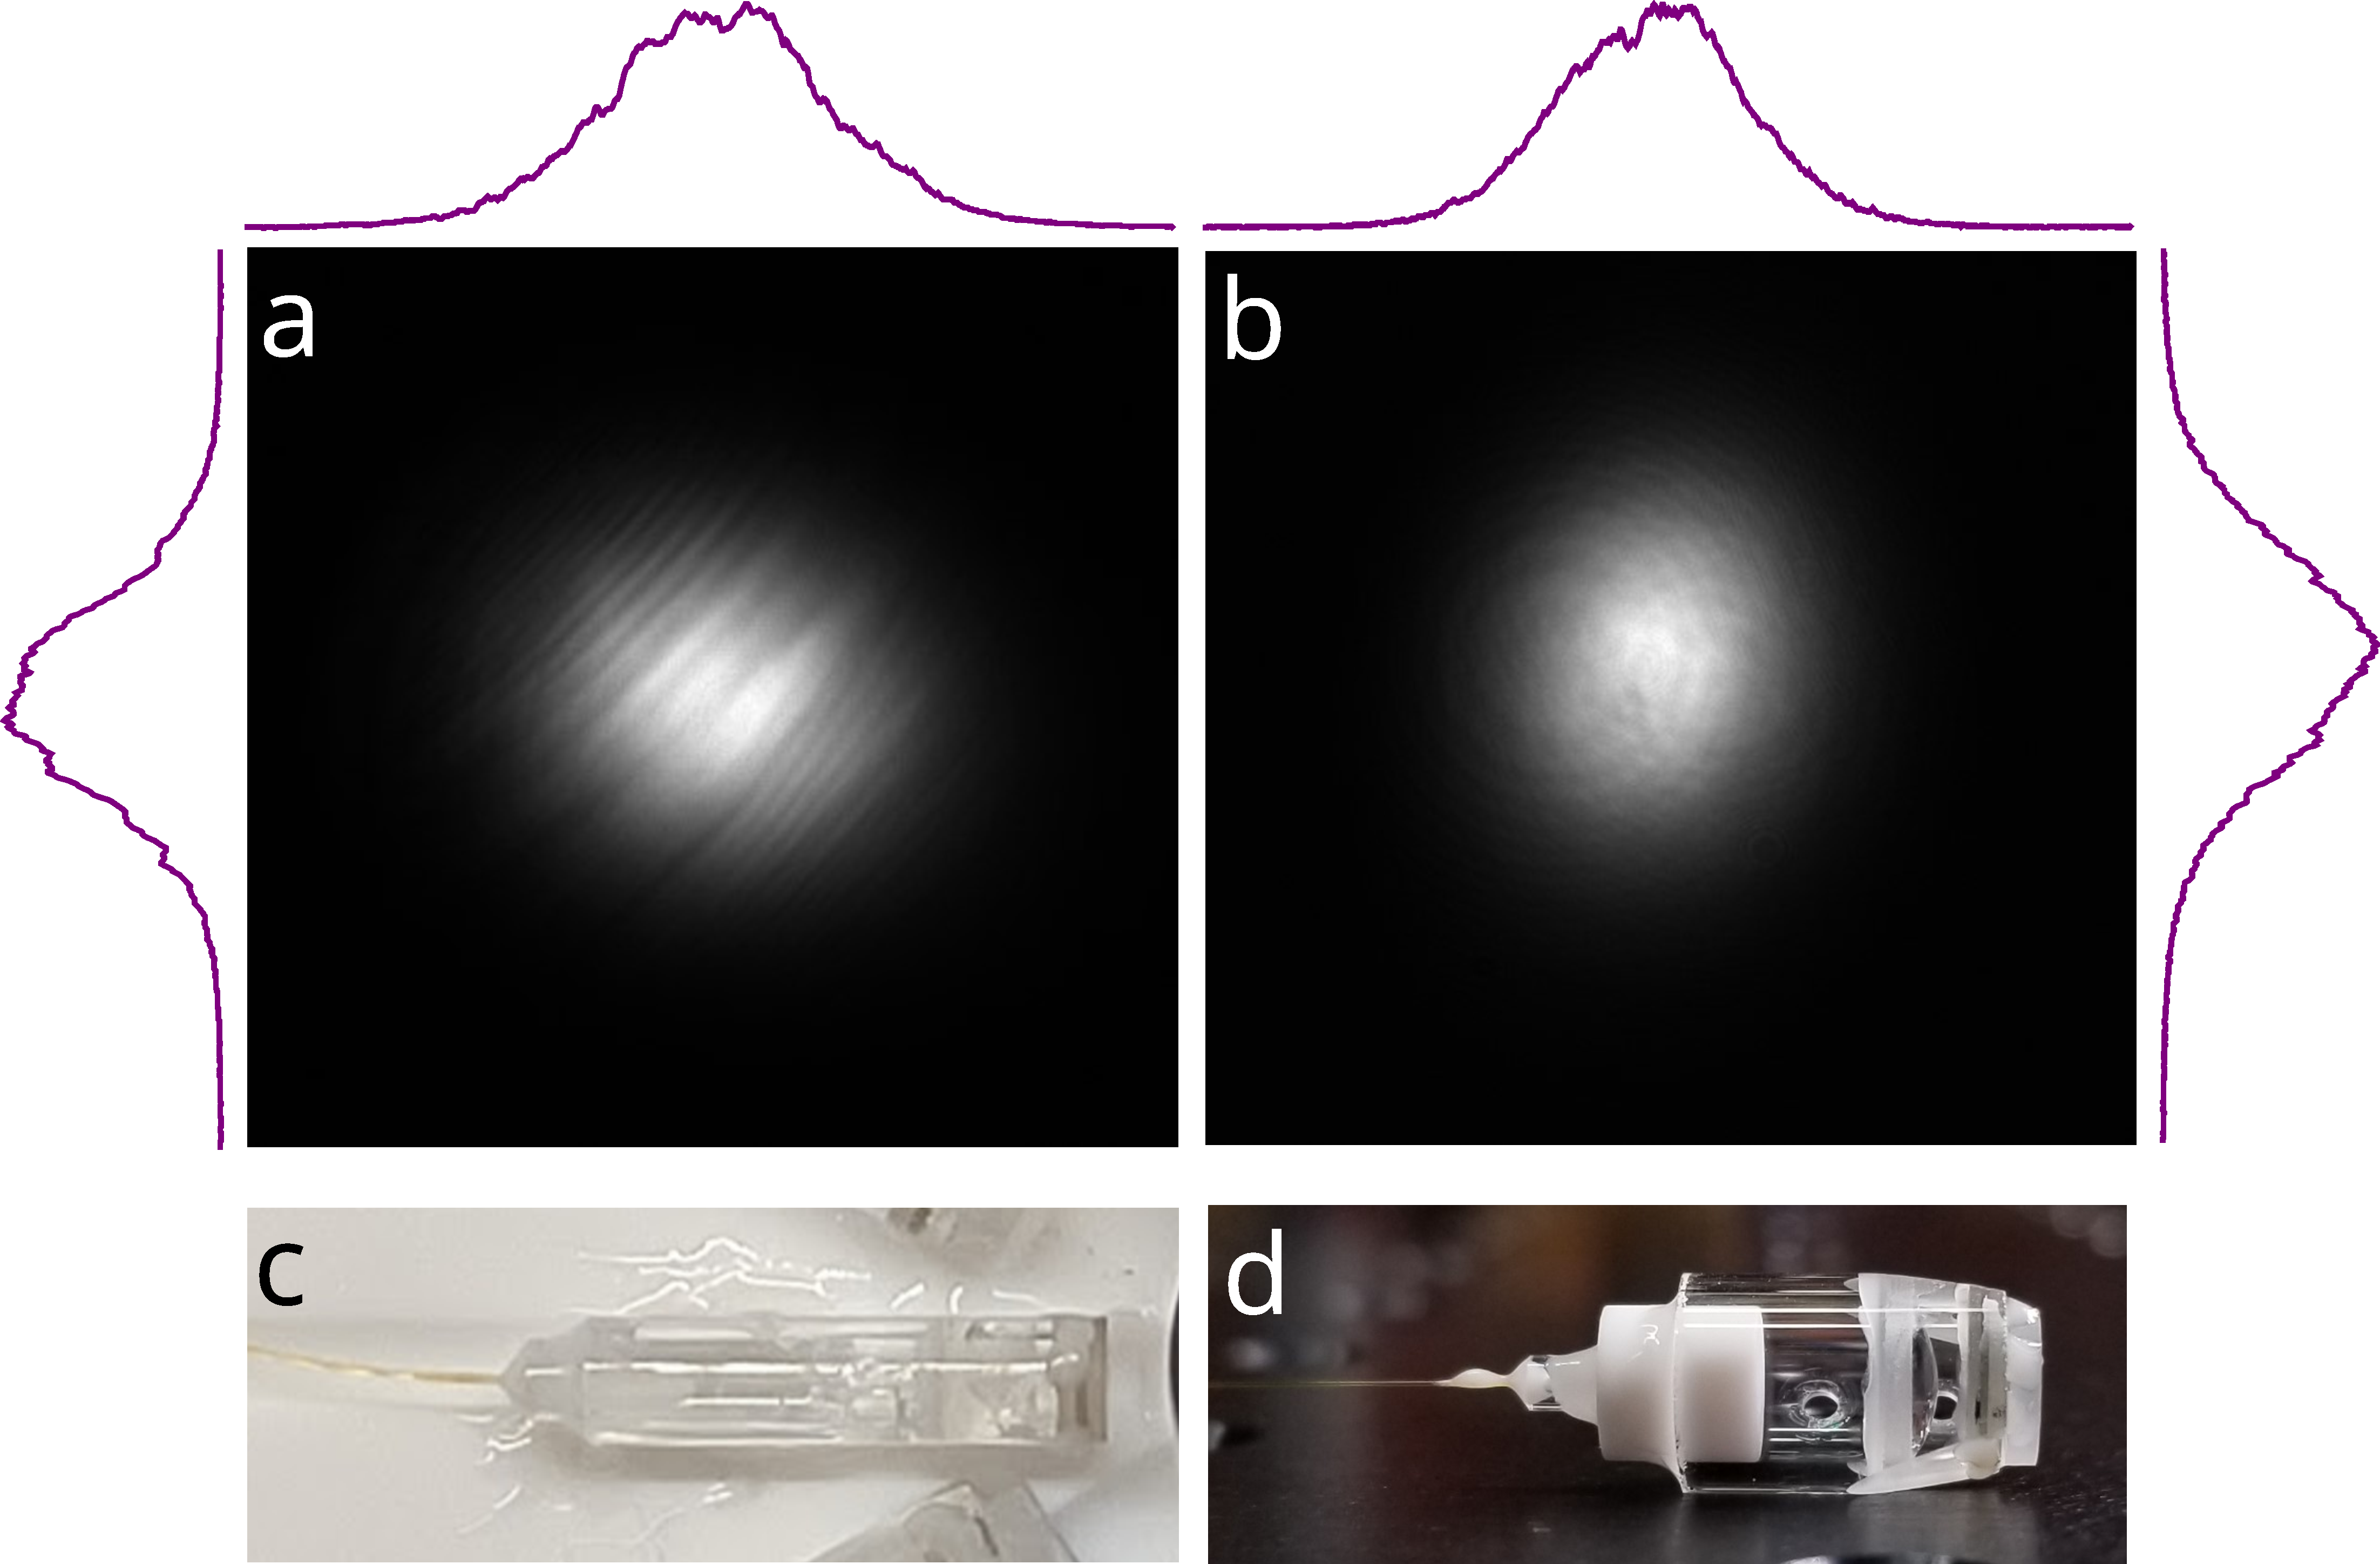
\includegraphics[width=0.8\textwidth]{Images/MOT_and_GRIN_tubes.pdf}
    \caption{Photos of assembled optical modules and their resulting beam profiles. The beam profiles shown are from \textbf{a} GRIN 2 and \textbf{b} MOT 1. The purple curves are cross sections of the beams. A typical MOT and GRIN tube are shown in \textbf{c} and \textbf{d} respectively. Although the quality of the beam produced by the GRIN lens is much worse than that produced by a standard glass lens of uniform refractive index, because the atom will be confined to an area of order $1 \mu$m$^2$, this aberrated beam profile is expected to be inconsequential.}
    \label{fig:assembled_optical_tubes}
\end{figure}

\subsection{Parabolic mirror: dipole trap and photon collection}\label{sec:mirror}

\subsubsection{Mirror optics design}

In the first version of our quantum node design, photon collection and dipole trap were implemented with the same optical path, composed of an SM fiber (FiberCore SM800(4.9/125)P/001), an achromatic doublet (Edmund $\#$47-377), and a custom high-NA on-axis parabolic mirror (NiPro Optics). The fiber ferrule was mounted in a Macor ring, which in turn mounted into a machined Macor tube along with the lens and the mirror. The fiber was chosen to be SM, which affords the greatest flexibility, because the target photon emission from the atom will be $\sigma$ polarized, while the dipole trap light will be $\pi-$polarized. 

A parabolic mirror was chosen over refractive high-NA optics since reflective optics are inherently achromatic, allowing us to align the optics for both photon collection at 780 nm and a dipole trap near 852 nm simultaneously. The entire photon collection optical train is then nearly perfectly achromatic, as the doublet lens has much less than 1 $\mu$m axial chromatic shift between 780 nm and 852 nm light, as checked with Zemax OpticStudio. The custom mirror, manufactured by NiPro optics, is made of diamond-turned 6061 aluminum body coated with a protected silver coating. For dimensions of the mirror, see the mechanical drawing given in \ref{ch:mech_drawings}. The mirror was baked in air by NiPro up to 130 $^{\circ}$C, ramped at 2 deg/min, and held at this temp for 16 hours before ramping down, to ensure that the coating would not peal off at this temperature. The mirror was designed to have a working distance of 5.26 mm and clear aperture NA of 0.61, corresponding to over 14$\%$ collection efficiency, given by,
\begin{equation}
    \eta = 2\pi\int_{0}^{\sin^{-1}(\text{NA})} E_{\sigma_{\pm}}(\theta)^{\ast} \cdot E_{\sigma_{\pm}}(\theta) d\theta 
\end{equation}

for $\sigma$ light if the quantization axis is taken to be along the axis of the mirror. $E_{\sigma_{\pm}}$ is the probability density function for circularly polarized emission from a radiating dipole as pattern as a function of emission angle. This collection efficiency does not, however, tell how much of the light can be coupled back into a single mode fiber. The finite aperture of the mirror is comparable to the diameter of the ideal Gaussian mode for mode matching to the SM fiber. The mirror also has a central through hole, explained below. To estimate the collection efficiency into a single mode fiber, the system was modeled in Zemax OpticStudio, with the atom approximated as a point source emitting rays isotropically into the solid angle spanned by the mirror. This calculation predicts a coupling efficiency of $78\%$ into the SM fiber.

The mirror has an on-axis through-hole of 0.5 mm diameter to allow collimated dipole trap light to pass through. This allows for tuning the degree of linear polarization of the dipole trap by maximizing the light transmitted through a linear polarizer placed behind the mirror and coupled out of the vacuum system with an optical fiber. An optical module was constructed for this purpose, which is the same as one of the MOT tubes except that it lacks a quarter waveplate, and is terminated with a multi-mode fiber (Thorlabs UM22-200) to maximize the amount of light coupled out of the system. In the experiment, we can monitor and maximize the dipole trap light coupled into the MM fiber, using waveplates before the SM fiber which sends the light to the mirror. This allows us to tune the dipole trap to be linear, though we note that this only provides a starting point for tuning the polarization. For a tightly focused dipole trap, the collimated input light should be slightly elliptical to minimize heating in the trap \cite{Garcia2018}. 

\subsubsection{Alignment and characterization}

Aligning an on-axis mirror presents a significant challenge, as the focal spot cannot easily be viewed directly without obstructing the beam incident on the mirror. Additionally, because of the high NA of the mirror, tilt of as much as 0.05 degree can introduce significant coma, as checked in Zemax OpticStudio. In order to aid in alignment, the tolerance between the mirror and Macor tube was specified at less than 40 $\mu$m (a compromise to allow for the larger thermal expansion of the aluminum compared to Macor) and the mirror body was made to be 12 mm long, 10 mm of which sit in the Macor tube. This essentially guarantees that the mirror body is well-oriented to the tube axis. 

A tapered fiber can be used as an approximate point detector, by coupling light into the fiber tip and measuring the output at several coordinate points in space to directly measure the shape of an optical intensity pattern \cite{TOLEDOCROW1995,RHODES1998}. In this way, we were able to directly map the focal intensity pattern produced by the mirror. The width of the cladding on the tapered fiber used (K-Tek Nanotechnology E50-780HP, uncoated tip) was only 125 $\mu$m, such that the length of fiber extending in front of the mirror, equal to the radius of the mirror or 4.1 mm, does not obscure a significant fraction of the light incident on the mirror. The fiber tip was held and moved using a piezo stage (Thorlabs NanoMax 603D) controlled by a LabVIEW program to take 2D raster scans of the field and record the signal out of the fiber with a photodetector (Thorlabs APD430A) at each positional step. 

To align the mirror, doublet, and fiber, the fiber-ferrule assembly and doublet were inserted into the Macor tube and adjusted to give a collimated beam at 780 as verified with a shearing interferometer. The fiber and lens were both held with custom 3D printed fixtures held by a 3-axis translation stage with 2-axis tilt and 2-axis rotation stage, respectively. The fiber assembly was tilted to steer the beam to propagate roughly along the axis of the mirror tube. The mirror was then inserted into the Macor tube and glued in place. The fiber tip was moved into the approximate location of the focal field by eye, sometimes by observing the scattering of 780 nm light off the end of the fiber. About 15 mW of light on the mirror, and the observed coupling efficiency into the fiber tip was on the order of $10^{-5}\%$. The remainder of the alignment was done by iteratively making an adjustment to the tilt of either the fiber or doublet, and running the raster scan code to see the current shape of the focal intensity pattern.

\begin{figure}
    \centering
    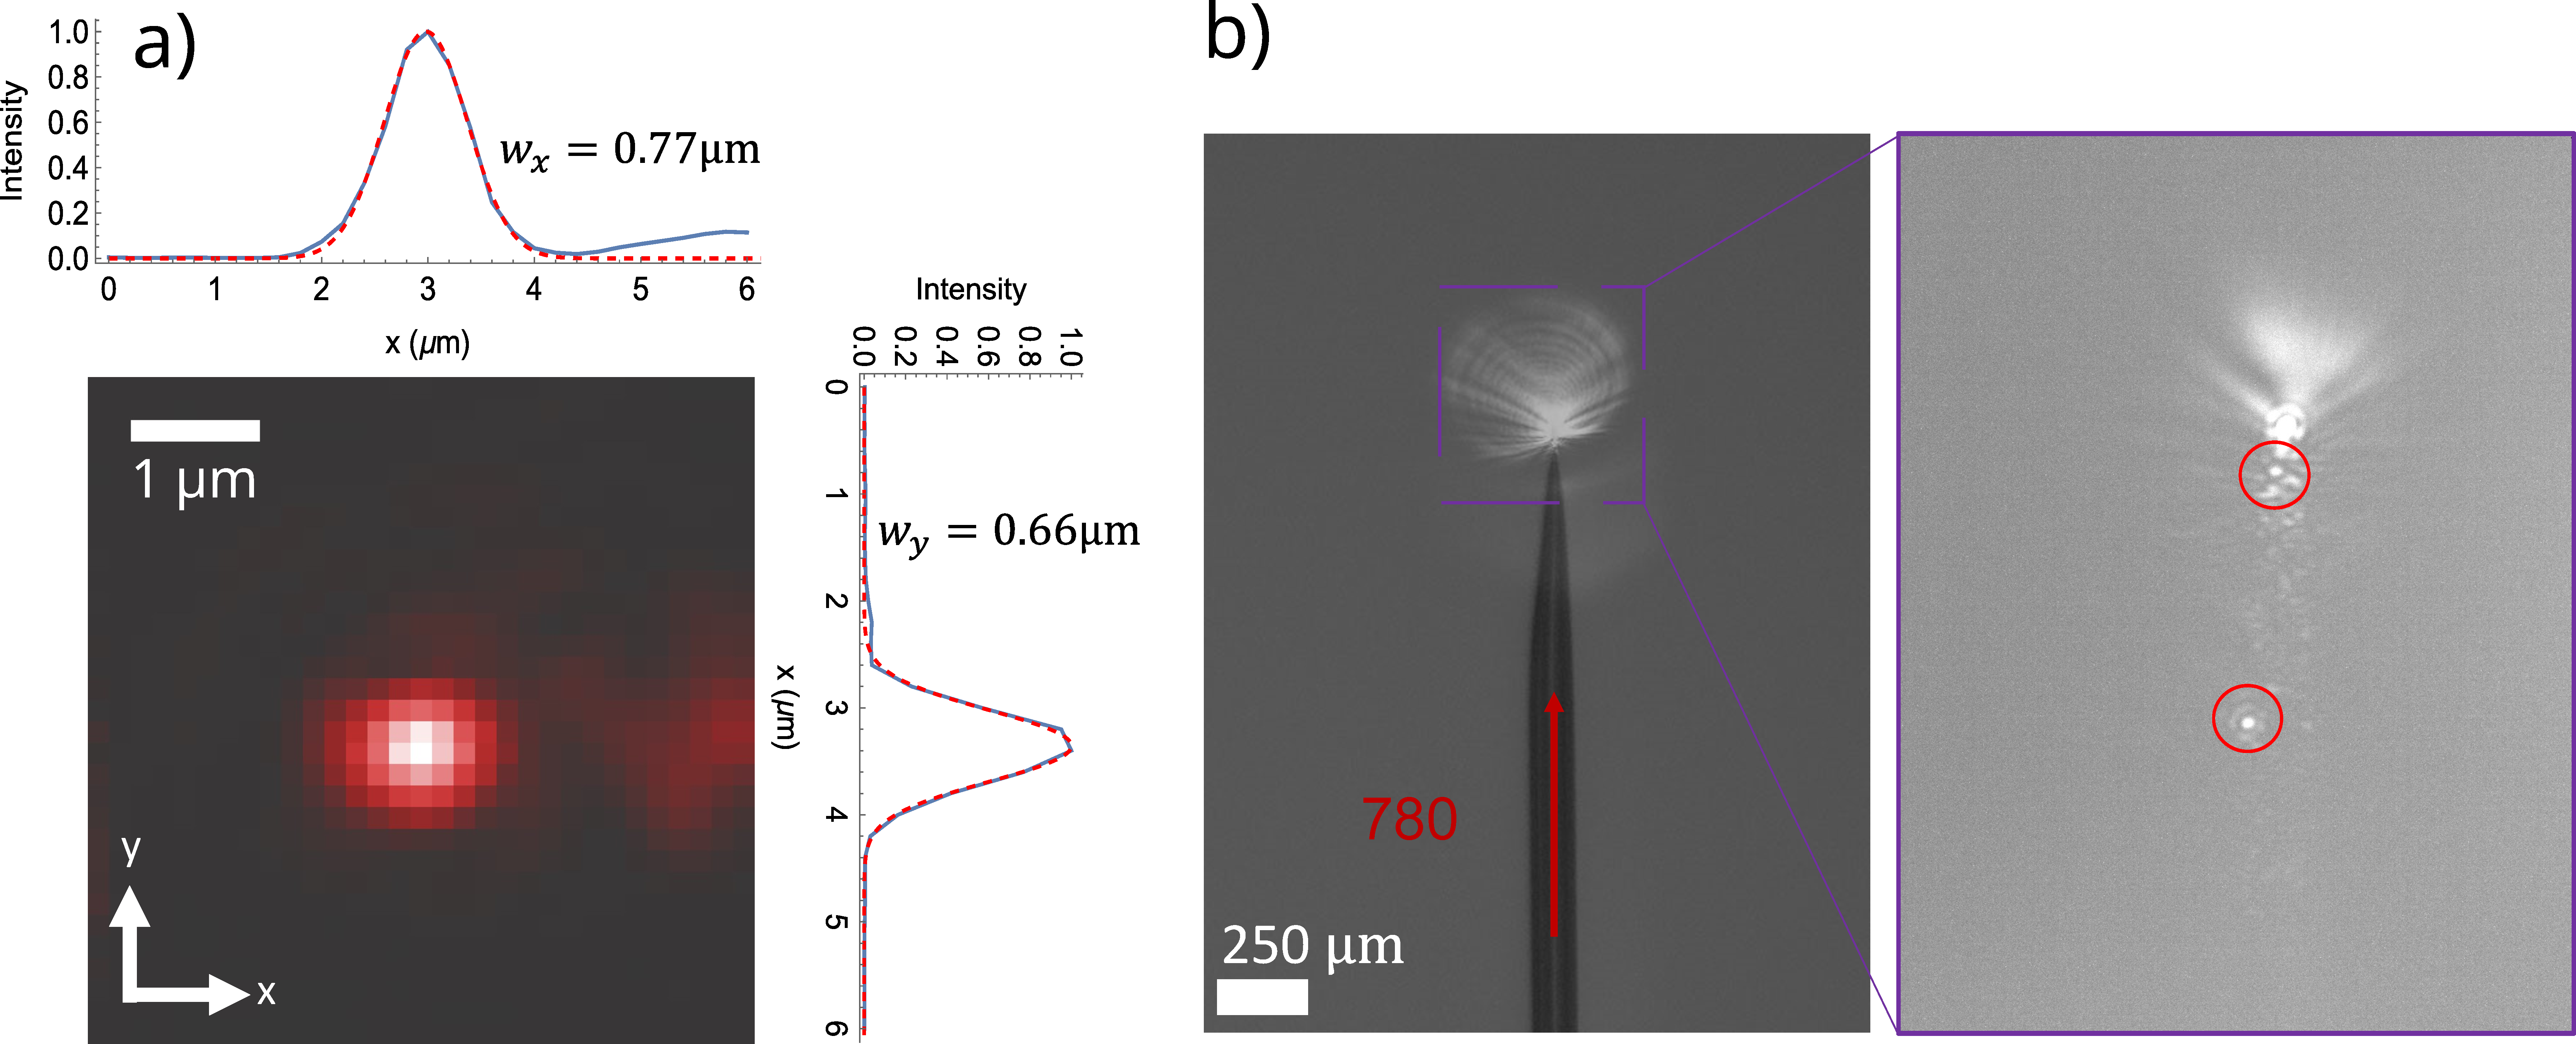
\includegraphics[width=\textwidth]{Images/mirror_focus_fiber_scan.pdf}
    \caption{\textbf{a)} The mirror focal intensity pattern as measured by coupling light from the mirror into a tapered fiber tip with a raster scan. Gaussian fits are shown for slices in $x$ and $y$, where the fiber tip pointed along $-y$. The step size of the scan was 200 nm in each direction. The apparent aberrations on the beam are due to coupling into defects in the fiber tip, shown in \textbf{b)}. By coupling light into the non-tip end of the fiber, we can see that the emission, and hence collection, mode shape is not truly point like. The left and right images show the fiber with lower and higher exposure and zoom, respectively, to make clear the structure of the tip mode (left) and the weaker defect modes (right).}
    \label{fig:mirror_fiber_scan_post_gluing}
\end{figure}

The image of the focal intensity pattern, after optimizing the alignment and gluing the fiber assembly and doublet, is shown in Fig. \ref{fig:mirror_fiber_scan_post_gluing}. The fitted $1/e^2$ Gaussian waists are $w_x=0.77~\mu$m and $w_y = 0.66~\mu$m, where x and y are the along the fiber axis and perpendicular to the fiber, respectively. These values are within about $20\%$ of the diffraction limited value given by $\lambda/(2 NA)$. Note that the beam exhibits apparent aberration along direction x but only on one side of the beam. This is an artifact of weak coupling of light into defects in the stem of the fiber tip, which are shown in Fig.  \ref{fig:mirror_fiber_scan_post_gluing}b and was verified by rotating the mirror tube 90 degrees with respect to the fiber tip and repeating the scan, which shows that the aberrations show up in the same place with respect to the fiber tip. This second scan showed the aberrations in the same place with respect to the fiber, confirming they were not from the intensity pattern.

A full reconstruction of the three-dimensional shape of the beam focused by the mirror can be done using the tapered fiber. To approximate this, several transverse scans of the beam were taken, with 0.5 $\mu$m longitudinal (i.e. along the mirror axis) steps between each slice. The result is shown in Fig. \ref{fig:fiber_scan_axial_steps}, where it can be seen that the beam appears to distort and translate as it expands. This can be mostly explained by coupling of the light into the tapered fiber defects as well as a slight angle between the true axis of the beam propagation and the axis of the fiber longitudinal steps. 

\begin{figure}
    \centering
    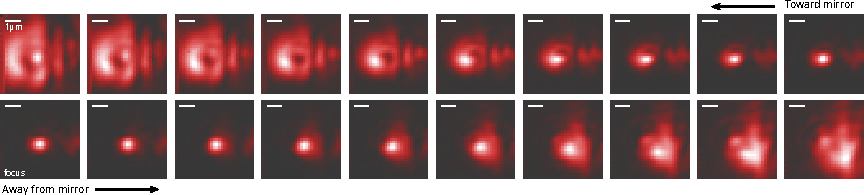
\includegraphics[width=\textwidth]{Images/fiber_scan_tranverse_slices.pdf}
    \caption{Transverse slices of the dipole trap beam taken at several axial positions about the focus. Each pixel is 200 nm and the longitudinal position varies by 0.5 $\mu$m between each slice. Note that each slice has been individually normalized for clarity.}
    \label{fig:fiber_scan_axial_steps}
\end{figure}

Additional fiber scans were done using 852 nm light to illuminate the mirror, in order to verify the expected low chromatic shift between the emitted photon light at 780 nm and the dipole trap light. However, it was observed that the tapered fiber position drifted monotonically on the order of 100 nm over a minute while we were making some of the measurements, such that subsequent raster scans in the same space showed an apparent drift the peak focal intensity. In order to characterize the difference in the positions of the focus at 780 nm and 852 nm even in the midst of this drift, we took a series of scans alternating between the two wavelengths at each scan. Because the drift was primarily along one axis of the available scan degrees of freedom, we were able to scan such that the drift would be confined in that the plane and we could repeat the scans without changing alignment between them. The results of this series of measurements is shown in Fig. \ref{fig:780_852_fiber_scan}. By fitting the drift of the focus along $z$ at each wavelength individually, we find an average difference of 72 nm between the $z$ positions of the focus at the two wavelengths over the hour scan time. In the other transverse direction, $y$, we infer a difference $<$ 200 nm, which is the resolution of the scan in this direction. Finally, we infer an axial chromatic shift of $<$ 500 nm.  

\begin{figure}
    \centering
    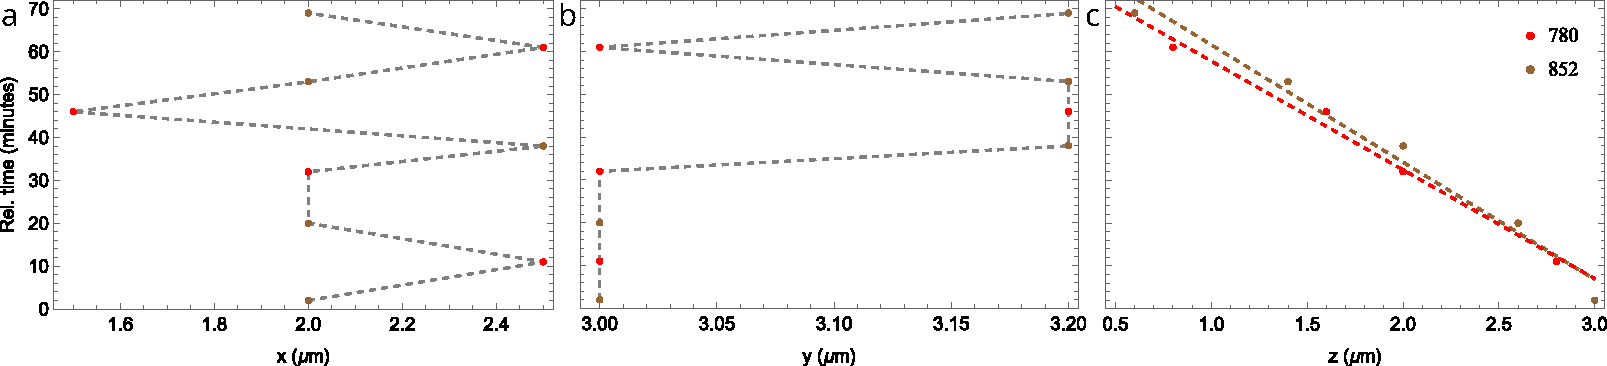
\includegraphics[width=\textwidth]{Images/fiberscan_852_780_xyz_fig.pdf}
    \caption{Tapered fiber scan measurement of chromatic shift between 852 and 780 nm light focused by the parabolic mirror. \textbf{a}, \textbf{b}, and \textbf{c} show the coordinate of the brightest pixel for a given 3D scan at either 780 (red points) or 852 (brown points), at $x$,$y$, and $z$, respectively. In the lab frame, gravity points along $-\hat{z}$, the fiber tip points along $\hat{y}$, and the detected beam propagates along $\hat{x}$. In each 3D scan, the step size is 200 nm in $y$ and $z$ (i.e. in the transverse planes), and 500 nm in the axial direction. The dashed lines in \textbf{a} and \textbf{b} are guides to eye, whereas the dashed lines in \textbf{c} are linear fits to the data for each wavelength.}
    \label{fig:780_852_fiber_scan}
\end{figure}

\subsection{Co-alignment of the on-chip optics}

Once the optical modules had been assembled, they were aligned one at a time on the Macor chip. The location of a trapped atom in experiments will be within the focus of the parabolic mirror, which is a volume of order 1 $\mu$m$^3$ All of the other beams, which have comparatively much larger cross-sections, need to overlap the focal region of the parabolic mirror. Additionally, the pairs of counter-propagating MOT and excitation beams should have their k-vectors roughly anti-parallel. The polarization degree of freedom of the optical pumping beams also needs to be aligned with respect to the optical axis of the dipole trap. Because each additional optical model added to the chip introduces an additional blind spot, the order of operations to co-align the beams is critical. 

During the alignment process, a method was needed to view the focused spot of the mirror as well as the other, much larger beams, without significantly blocking light incident on the mirror. A thin flat semi-transparent sheet with negligible cross section compared to the area of the mirror could be used as a scattering surface, as shown schematically in Fig. \ref{fig:scattering_sheet_method}. We made a makeshift thin diffuser surface by rinsing a strip cut from a transparency sheet with acetone and subsequently blowing it dry with canned air, which created a uniform cloudy finish on one side. The sheet had a thickness of 80 $\mu$m and could be inserted through the central hole in the Macor bridge with the plane of the sheet coincident with the mirror tube’s optical axis. The rough positioning of the sheet, with the help of a 3-axis translation stage, was done by eye and with a camera looking down on the bridge from above. The stage also allowed for retracting the strip back down through the bridge to allow the beams to pass unobstructed as is necessary at various stages of the alignment.

\begin{figure}[t!]
    \centering
    
\includegraphics[width=\textwidth]{Images/beam_projection_imaging_schematic.pdf}
    \caption{Schematic of the setup to image the optical chip beams as projected on a transparent scattering sheet made from an acetone-rinsed transparency sheet.b  \textbf{a} Cross-section of the optical chip from the side showing the transparency sheet in the path of the beam incident on and reflected by the mirror, and the projection of a MOT beam (light red oval). \textbf{b} View of the optical chip and transparency sheet from the top, showing the imaging path. \textbf{c} A photo of the optical chip showing the transparency sheet. Inset \textbf{d} shows the transparency sheet which appears matte white after the acetone rinse, and inset \textbf{e} shows its surface under an inexpensive microscope, captured with the author's phone's camera. The apparent bulge is due to optical aberration.}
    \label{fig:scattering_sheet_method}
\end{figure}

It is worth noting a couple of technical points that constrained the way in which we aligned the optics. The machining tolerances between the cylindrical grooves on the Macor bridge and the tubes housing the optical components were of order 10 $\mu$m, which ensures that the optical modules should be close to the correct alignment for ``free” as soon as they are placed on bridge, with the exception of the parabolic mirror tube for which the axial degree of freedom must be adjusted. However, imperfection in either the placement of fibers and lenses in the tubes or imperfections in the lenses in themselves result in the beams traveling off axis or at slight angles to the axis of the of the machined grooves on the bridges, and these errors can only be corrected provided they are small. In particular, rotating the MOT beam tubes about their axis in the grooves allowed us to walk the beam position at the center of the bridge, typically by as much as 100 $\mu$m, but transverse positioning of the optical modules was extremely limited due to the close tolerances. 

To begin the alignment, both pairs of MOT tubes were placed on the bridge to check whether we could observe coupling of light output by one MOT tube into the fiber of the module opposite of it. One MOT tube was held in place with a 3D printed clamp using neodymium magnets above and below the Macor bridge, while the opposite MOT tube was rotated about its axis and poked by hand while the signal of a photodetector (TTI TIA-525) connected to the output fiber was observed on an oscilloscope. If no coupling was observed by moving only the unclamped MOT tube, the other was adjusted incrementally. Once coupling was observed with both pairs of MOT beams, it was verified that the beams were roughly aligned using a piece of matte Scotch tape as a scattering screen placed at the intersection of two beam coming one side of the parabolic mirror axis. None of the MOT tubes were glued in this preliminary check. Going forward, we will refer to the MOT tubes by numbers 1 through 4, as shown in Fig. \ref{fig:optical_chip_design}.

The science region, defined by the location of the mirror focus, was set by the intersection of MOT 1 and the mirror focus by axial adjustment of the parabolic mirror tube while viewing the overlap of the two beams on the transparency strip, as imaged through the side of the mirror tube with a zoom lens and CCD camera (ThorCam CS165MU1). MOT 1 was glued in place, in the position that it was left in after observing coupling to MOT 3 in the preliminary step, since it was not guaranteed that positioning the beam of MOT 1 to be exactly centered on the mirror would allow for coupling to MOT 3, which guarantees sufficient alignment of this MOT beam pair. For gluing of MOT 1, the mirror tube, and all other components below, the epoxy was applied in a small amount with a thin piece of solder used an applicator such that the applicator would be more likely to bend than to misalign the optical being glued if too much force was applied. UV light (UV wand model?) was applied for at least 60 s to each glued region.

Next, GRIN 2, situated on the same side of the mirror tube as MOT 1, was aligned. For this beam, the polarization alignment mattered as well as the position, such that free rotation of the optical tube to walk the beam to the best position was not possible. Due to space constraints on the bridge and the small diameter of the GRIN tube, it was not feasible to grab it with some kind of clamp while retaining sufficient freedom to move it. Instead, a 4 mm Thorlabs cage system rod was glued to the top of GRIN 2 after first roughly aligning the polarization. This rod, held by a 6-axis stage (3 translational d.o.f., 3 rotation), could then be used to precisely align both the position and polarization of the GRIN tube before gluing the tube in place and then gently breaking the rod free from the GRIN tube. This last step was confirmed to work in advance with a spare GRIN tube, rod, and Macor bridge to ensure the glue joint between the Macor and glass would win over the glass to steel joint. The 6-axis stage was constructed from off-the-shelf optomechanics.

The alignment of the polarization of the optical pumping beams produced by the GRIN tubes, relative to the photon collection axis, is critical. In many cold atom experiments, the optical pumping fidelity can be optimized by tuning both the polarization of the light and modifying the angle of the quantization axis with the magnetic shim fields. However, the fidelity of the atom-photon superposition states we generate depends on our ability to collect only $\sigma$-polarized light into the optical fiber. That is, changing the angle of the magnetic bias field to optimize optical pumping fidelity to compensate for polarization misalignment will in general come at the cost of collecting unwanted $\pi$-polarized photons which lower the entangled state fidelity. 

To align the polarization of the GRIN tubes, we first assume that the photon collection axis lies in a plane parallel to the plane of the bridge, and use a PBS (Foctec 780 nm High Extinction PBS) sitting on the bridge to define the target polarization axis. The GRIN 2 beam was roughly aligned to transmit through the PBS, corresponding to polarization lying in the plane of the bridge, then glued to the 4mm cage rod. The transmission of the light through the PBS is insensitive to small changes in the polarization angle, so we employ a slope detection method for fine tuning. 

A slope detector was made consisting of  motorized rotation stage (Thorlabs K10CR1) holding a linear polarizer (Thorlabs LPNIR100), followed by a photodetector whose output went to an analog input device (NI 782602-01) which could be read by a LabVIEW program which also controlled the rotator. By rotating the polarizer $\pm 45^{\circ}$ about a central $\theta_0$ and taking the difference of the transmitted intensity at those endpoints, we can programmatically feedback to the position of $\theta_0$ to align the polarizer to the reference polarization, i.e. that of the light passing through the PBS. The error in this process, accounting for the uncertainty and repeatability of the K10CR1, is $\sim 0.02^{\circ}$. After $\theta_0$ has been set to within this uncertainty, the same method of slope detection can be used to align the GRIN beam polarization with the PBS removed from the bridge. In this step, the polarization is manually adjusted in between the polarization measurements. The angular error, when it is small, can be estimated from the intensity difference at $\pm 45^{\circ}$ as $\delta \theta = -2(I(45^{\circ}) - I(-45^{\circ}))$. 

After aligning the polarization of GRIN 2 using the above method, the position was tuned to overlap the parabolic mirror focus on the transparency strip as best as possible within the mechanical constraints of the bridge. The final polarization error was measured to be $0.05^{\circ}$ after gluing.

For GRIN 1, we were not able to directly measure the polarization of the beam, since it gets blocked by GRIN 2. Instead, we aligned a polarizer on the bridge near where the end of GRIN 1 will go, using the method described above with the beam output by GRIN 2 as the reference polarization. The polarizer was roughly aligned to maximally transmit the GRIN 2 beam, then placed in a small amount of uncured glue on the bridge and poked into alignment with a tweezer by hand until the error could not be further reduced. The final error measured after gluing was $0.2^{\circ}$. 

To install GRIN 1, the ThorCam was pointed anti-parallel to the MOT 1 beam axis, from the MOT 3 side. Using the transparency sheet method, GRIN 1 was aligned to maximizing both the overlap with the parabolic mirror focus and the amount of light transmitted through the polarizer glued in the last step, since GRIN 1 has a polarizer glued to its output.

Projections of the images of the individual beams on the transparency sheet, made by summing the rows and summing the columns, show the extent to which the beams are co-aligned. This analysis is shown for three combinations of beams in Fig. \ref{fig:final_beam_projections}, including all beams except MOT 3, which blocked the imaging path once installed. MOT 3 was installed and aligned by coupling light from MOT 1. It is clear that the parabolic mirror focus is closer to the plane of the bridge than the centroids of the other beams. Nevertheless, because the other beams are much larger than the mirror focus we did not anticipate this being an issue. 

\begin{figure}[t!]
    \centering
    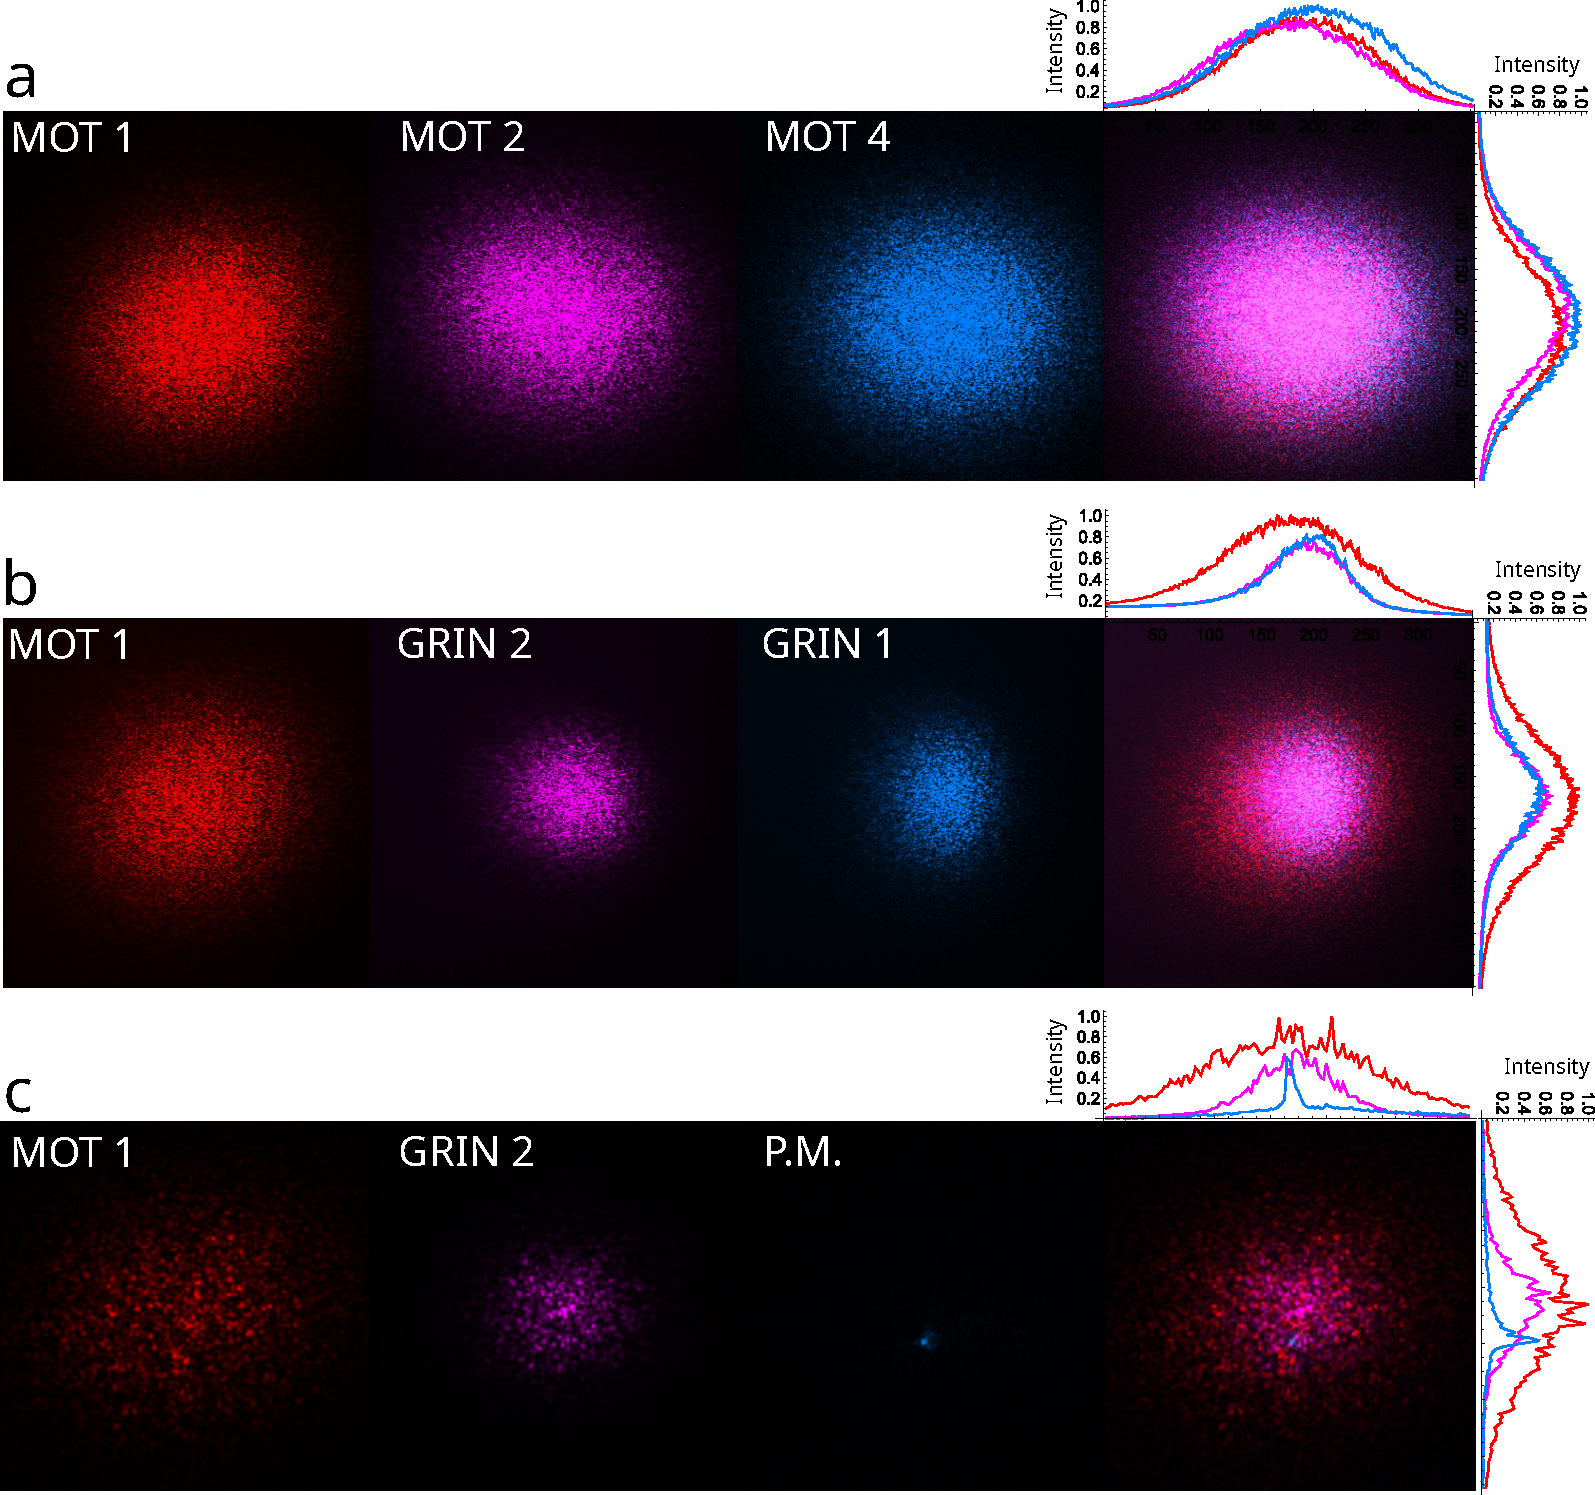
\includegraphics[width=\textwidth]{Images/transparency_sheet_beam_projections.pdf}
    \caption{Optical chip beam projections on an acetone-rinsed transparency sheet. A setup of the imaging schematic is given in Fig. \ref{fig:scattering_sheet_method}. The three panels \textbf{a}-\textbf{c} show different combinations of beam images, where the right-most image in each row is a combined image from the three individual beam images. The curves on the top and right sides are the sums of the rows and columns, respectively, for the individual beams. The ``P.M." image in \textbf{c} shows the focus of the parabolic mirror.}
    \label{fig:final_beam_projections}
\end{figure}

Lastly, an optical module for optimization of the degree of linear polarization of the dipole trap light was installed behind the parabolic mirror. Slope detection was not possible for this configuration. Instead, the same PBS used earlier was placed on the bridge behind the mirror and the polarization state of light coupled into the parabolic mirror SM fiber was tuned with free space waveplates to maximize the light transmitted through the PBS, corresponding to vertical polarization with respect to the bridge. The PBS ports were monitored to verify that the polarization state was not changing over several hours. Then the polarization module was aligned on the bridge by rotating about its own axis to maximize the light coupled out of the MM fiber before gluing this final module in place.

Finally, we note a couple of unexpected barriers that were encountered during the assembly described above. First, some excess cured epoxy on the parabolic mirror tube near the doublet lens prevented it from sitting correctly on the bridge. To remedy this, we removed some material from the bridge using a Dremel with a standard grinding attachment. Second, the epoxy used for gluing the last few optical modules to the bridge, which must be kept frozen when not in use, seems to have expired prior to the date. This was probably due to its being shipped without insulation or dry ice, as had been done with an earlier shipment we received. We realized that the epoxy was expired by noting that UV was not turning the glue completely hard to the touch. However, in the interest of not waiting a few more months for new glue, we modified our glue curing procedure. Following the standard minute-long exposure to UV, which partially hardened the glue, we applied a heat gun with a directed flow at 150 $^{\circ}$C to the glued area. 

\subsection{Optical chip installation and vacuum bakeout}
Following the gluing of the optical modules, the bridge was installed in the chamber and some final diagnostics were performed prior to completing the vacuum system. Installing the optical chip inside the science chamber was a formidable challenge of its own, largely because of the fragility of the fibers. In particular, near the glue joints fixing the fibers to their ferrules, it is easy to snap a fiber, rendering the optical module unusable and irreparable. This happened once while installing one of the GRIN tubes, and other times during the construction of the optical modules. To reduce the possibility of breaking fibers while installing the optical chip in the chamber, the fibers were strain-relieved to the Macor bridge with additional epoxy, after first bending the fibers to fit within the chamber. This step was done with the use of a bendable 3D-printed guide to mimic the perimeter of the inner wall of the chamber, which was safer than working with the chamber itself. We note that the bending radius for the fibers used is about 1 cm, and the optical chip layout was designed to satisfy this, albeit marginally. 

\begin{figure}[h!]
    \centering
    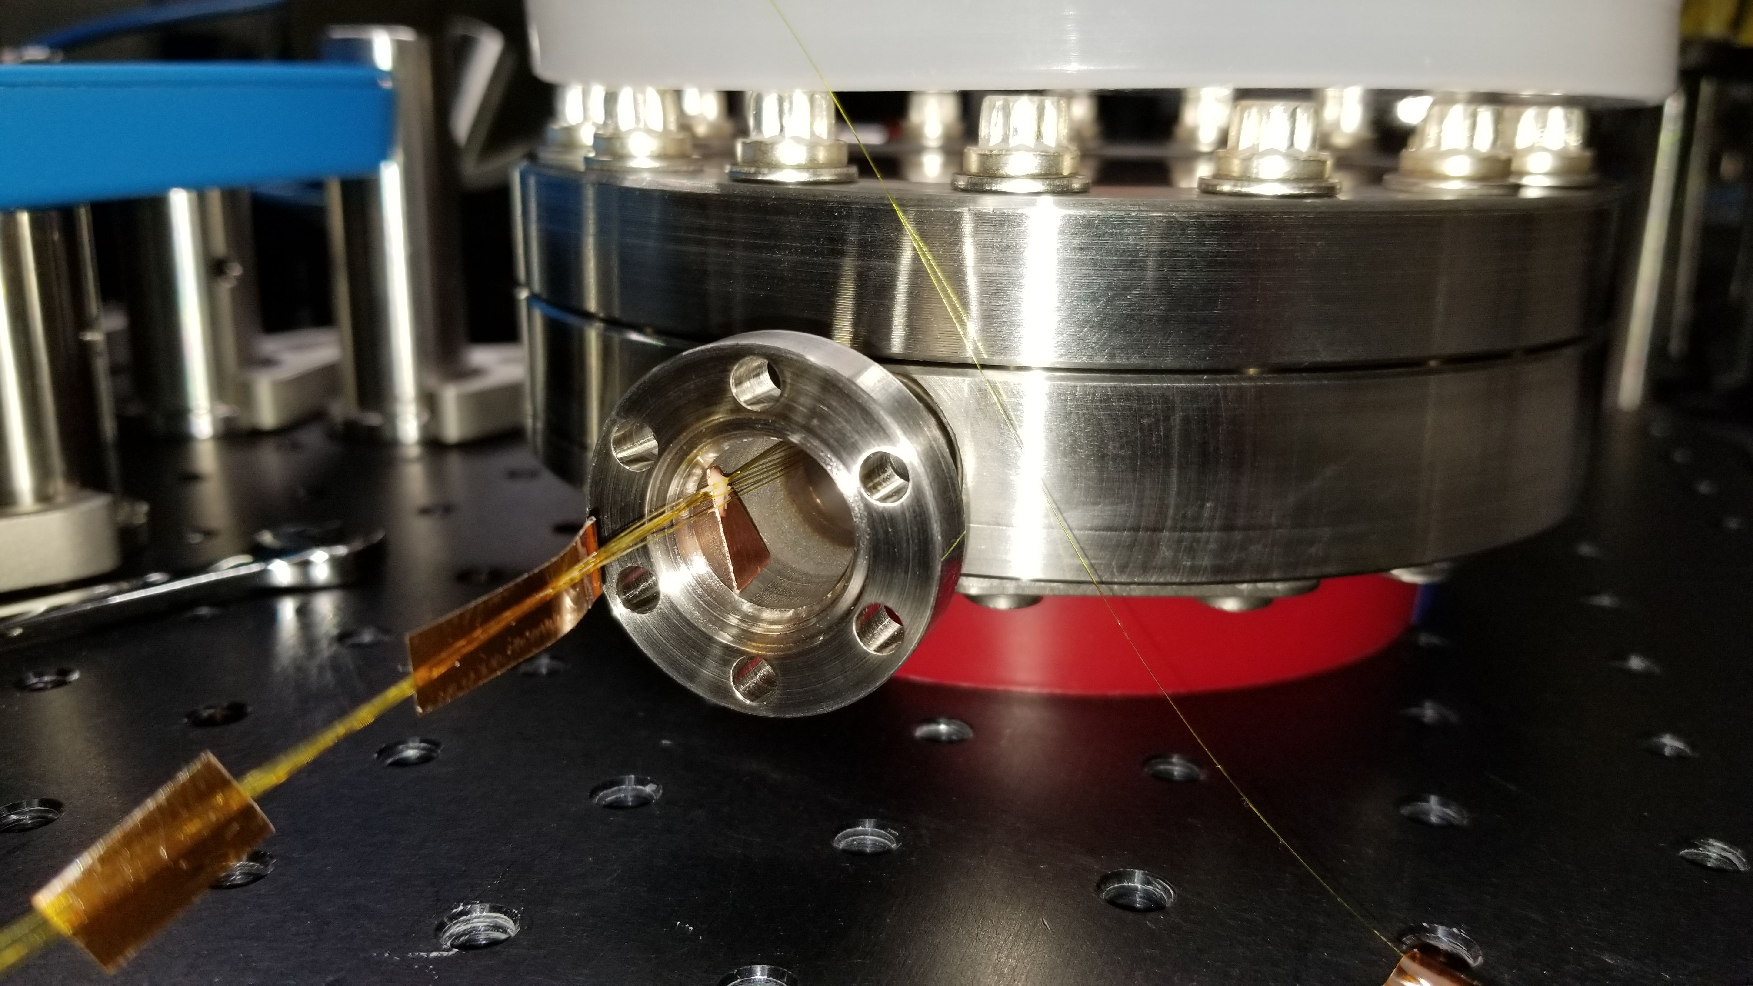
\includegraphics[width=0.7\textwidth]{Images/chamber_fiber_strain_relief.pdf}
    \caption{The optical fibers passing through the neck of the chamber were strain relieved by gluing a piece of the copper sheet to the chamber neck and gluing the fibers in turn to the copper. Note also the pieces of Kapton which can be seen securing the fiber bundle which is emerging from the chamber neck.}
    \label{fig:chamber_neck_strain_relief.pdf}
\end{figure}

To install the optical chip in the lower half of the science chamber, the fibers were fed through the neck of the chamber. This was done by first bundling the eight fibers together, secured with a small piece of Kapton roughly every 10 cm, so that they could be pulled through the chamber as a unit. The height of the optical chip in the chamber from the bottom window was set using copper spacers on each groove grabber, and clamped to the groove grabbers using copper strips and nominally non-magnetic stainless steel nuts and bolts. The nuts and bolts were observed to be very slightly magnetic, but apparently no more than the stainless steel vacuum components themselves. Finally, the fibers were strain-relieved in the neck of the chamber using a strip of copper sheet which was glued at one end to the neck, and to which the fibers were glued to the other end (Fig. \ref{fig:chamber_neck_strain_relief.pdf}). This design had the intention of allowing us to remove the fibers if need be, with lower risk of breaking them compared to gluing the fibers directly to the chamber, by snipping the copper strip. The completed optical chip installed in the lower half of the science chamber is shown in Fig. \ref{fig:chip_in_chamber_akbar}.

\begin{figure}[h!]
    \centering
    \begin{subfigure}[b]{0.61\textwidth}
        \centering
        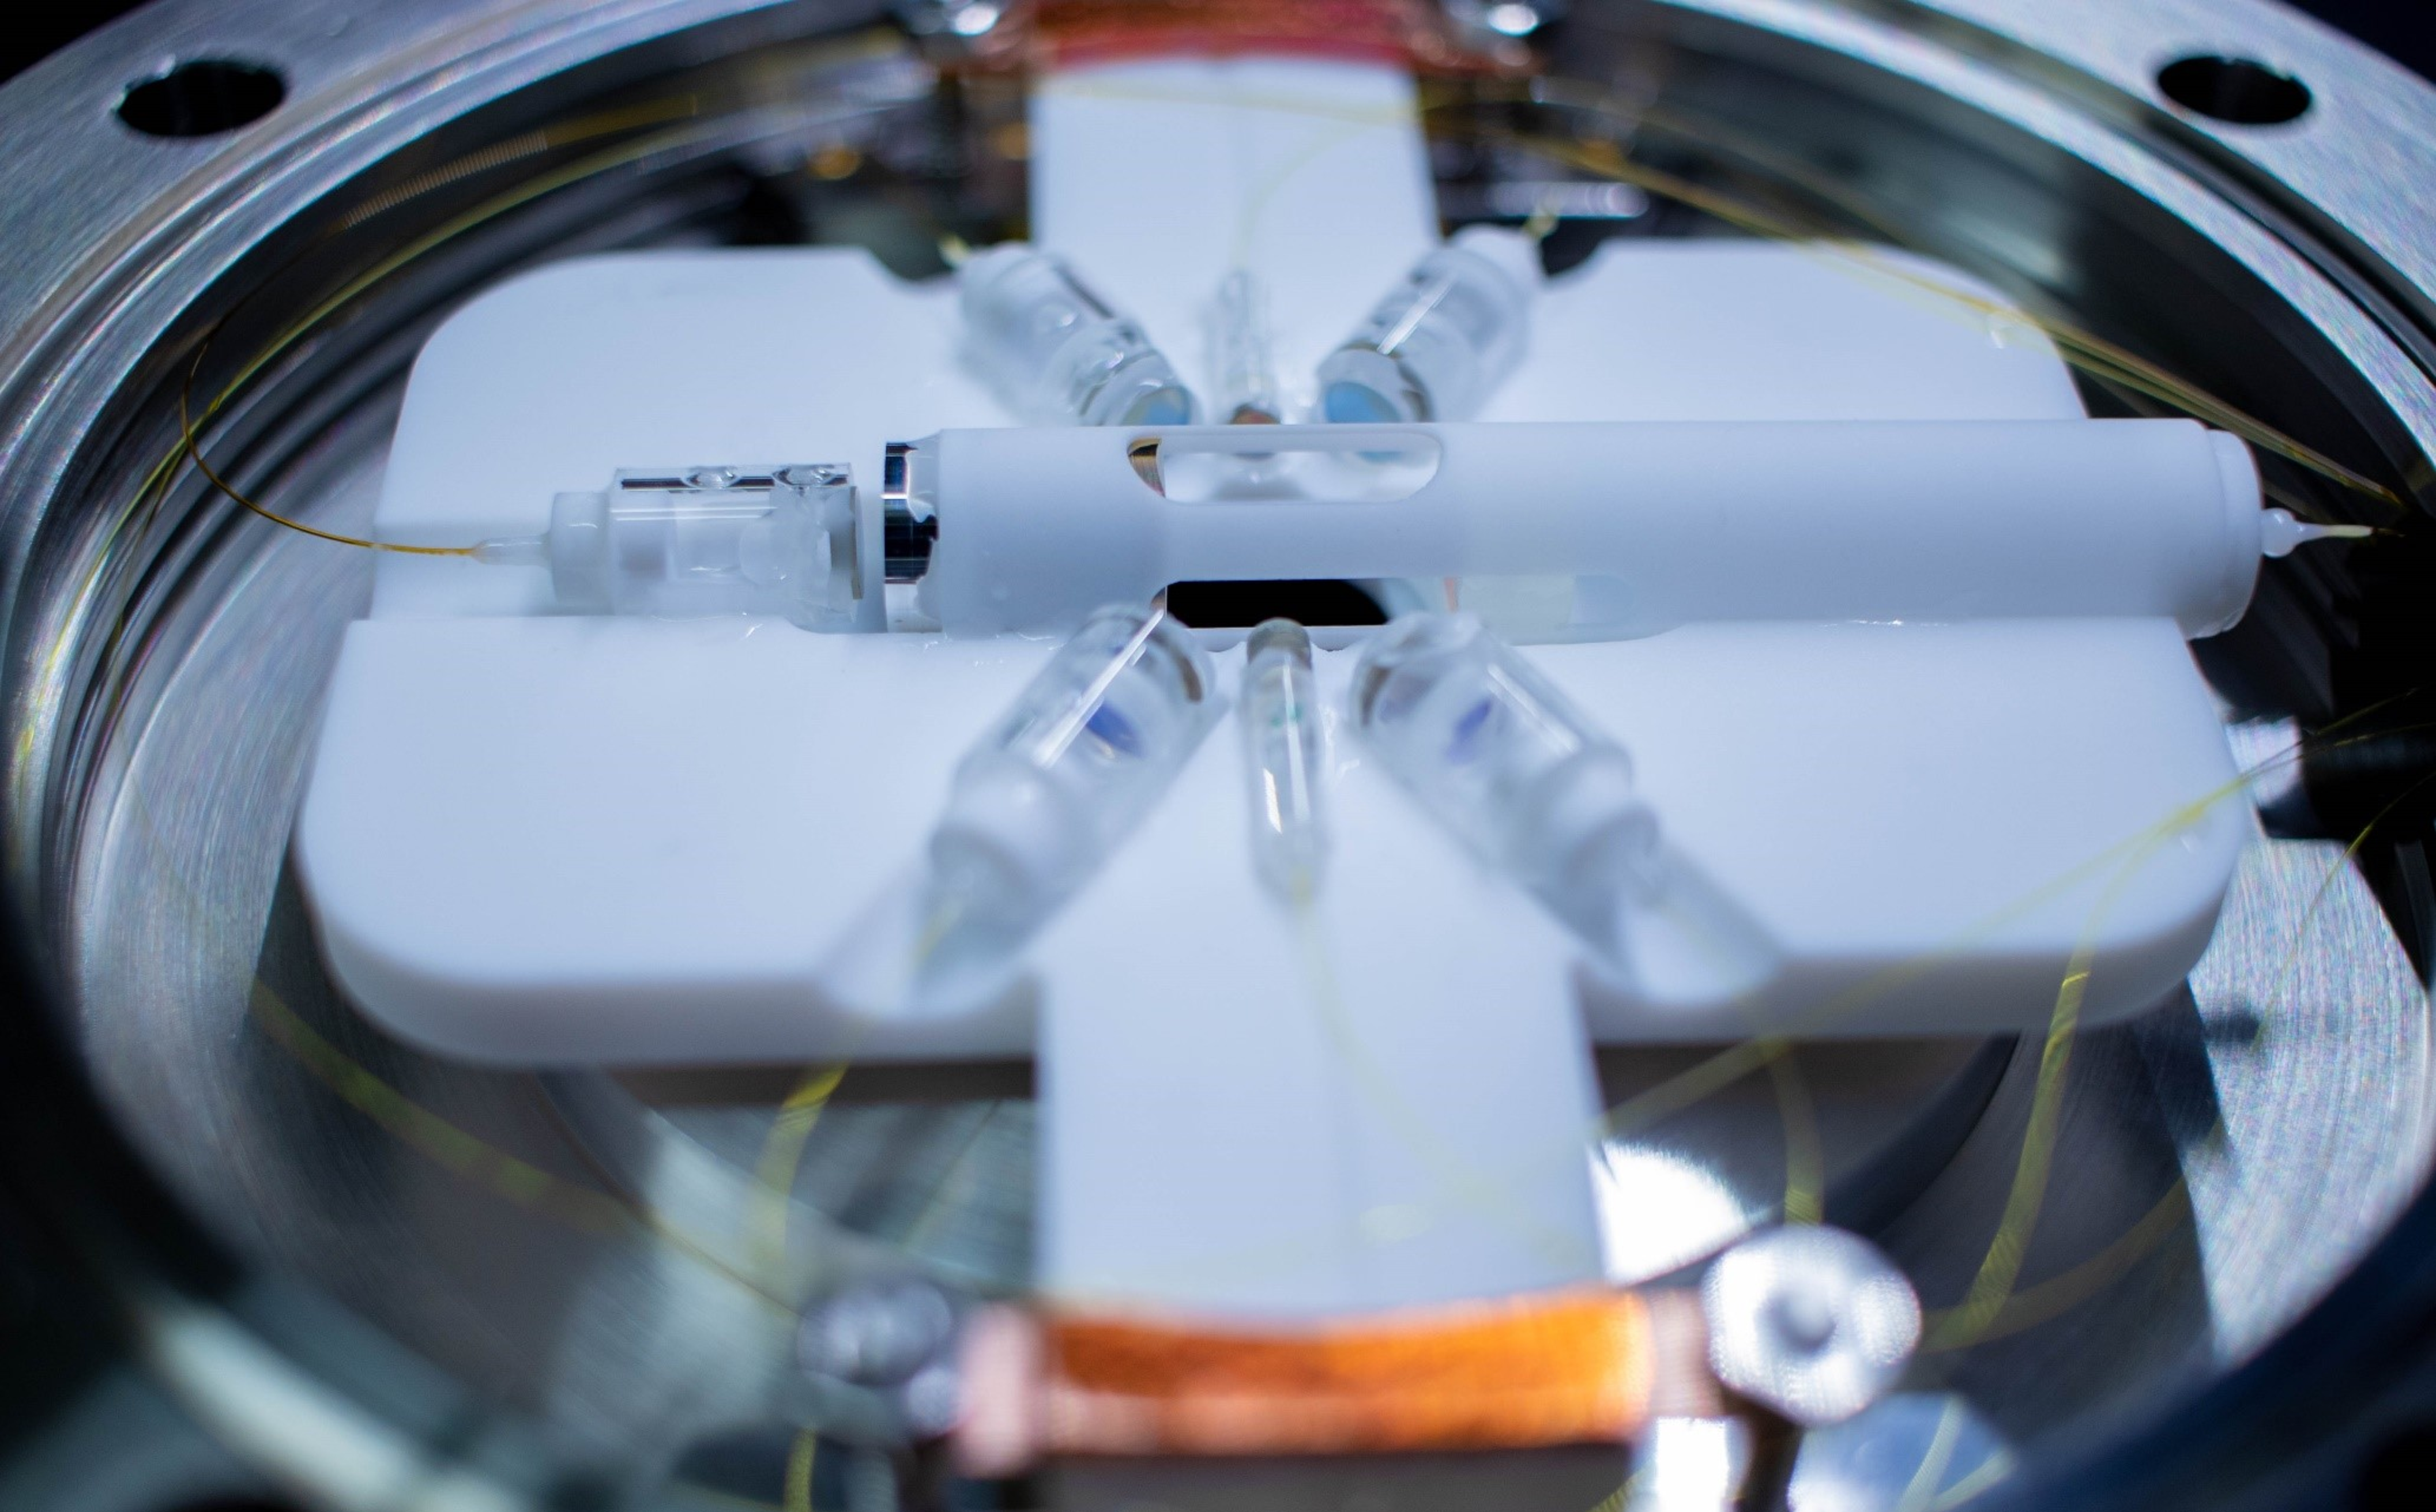
\includegraphics[width=\textwidth]{Images/chip_in_chamber_akbar.pdf}
    \end{subfigure}
    \begin{subfigure}[b]{0.375\textwidth}
        \centering
        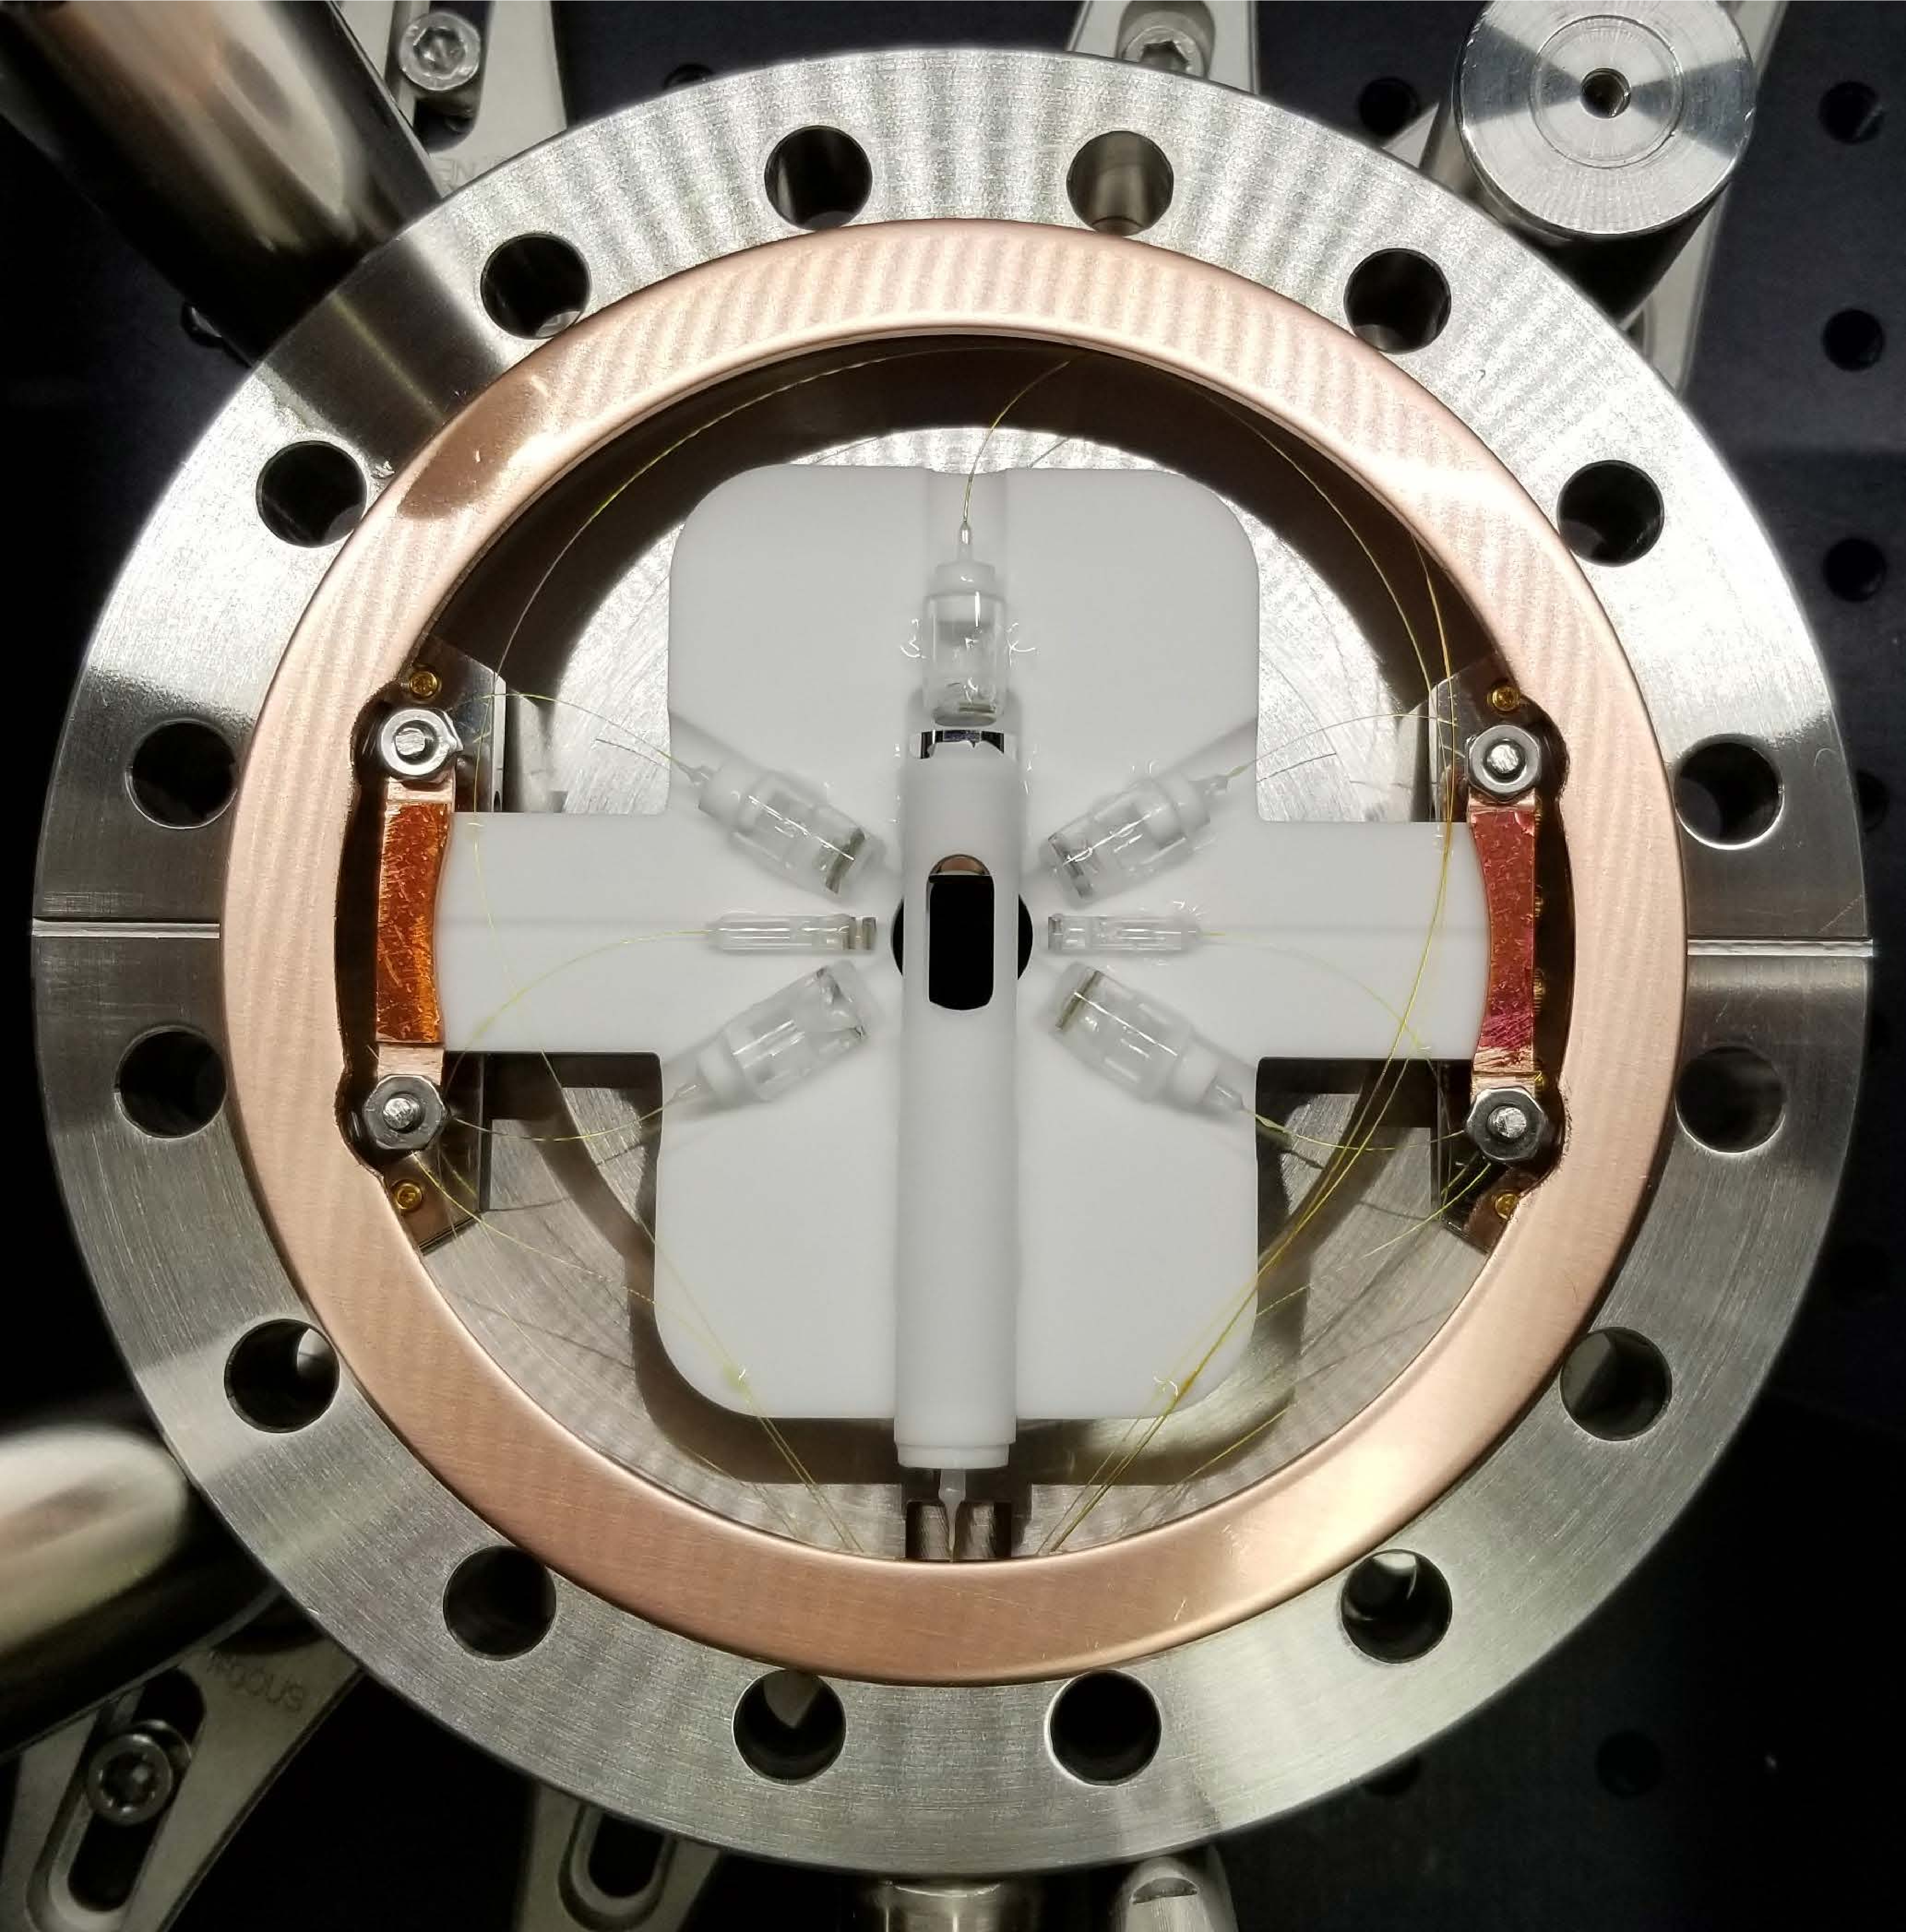
\includegraphics[width=\textwidth]{Images/chip_in_chamber_with_gasket.pdf}
    \end{subfigure}
    \hfill
    \caption{The finished optical chip in the science chamber, with the top of the chamber removed. In the right photo, note that the copper gasket has been cut to make clearance for the nuts which secure the bridge. Photo credit: Akbar Safari.}
    \label{fig:chip_in_chamber_akbar}
\end{figure}

As a final precautionary measure prior to installing the science chamber on the rest of the vacuum system, the chip was baked in air with the science chamber fully assembled. This was to ensure the glue, which can be cured with heat, was fully cured, allowing us to check the alignment of the optics a final time before the vacuum bake out. The chamber was ramped up to about 120 $^{\circ}$C at a rate of roughly 0.4 deg./min, and held at over 110 $^{\circ}$C for over an hour before being ramped back down to room temp. 

To check the final optical alignment after the air bake, the top of the chamber was removed and we mapped out the field of the beams using the tapered fiber scanning method described earlier. This time, we used a Femto FWPR-20-SI detector, which afforded us the sensitivity needed to detect light from the MOT and GRIN beams using only ~ 1 mW of injected power. A raster scan, as described in Sec. \ref{sec:mirror} was first used to verify that the shape of the parabolic mirror focal intensity had not become aberrated. Then, by first parking the fiber at the peak intensity of the mirror focus, a series of scans were done to check the relative positions of each beam with respect to the mirror focus. For MOT 1, MOT 4, GRIN 1, and GRIN 2, two 1D scans each were done, with one scan direction along the mirror optical axis, y, and the other, z, direction perpendicular to the Macor bridge. Scans were not done for MOT 2 and MOT 3, as coupling from 1 to 3 and from 4 to 2 was measured to be at least 7$\%$ and 2$\%$, respectively. Note that the actual coupling may be higher by a factor of two or so. This is because the light was butt-coupled into MOT 1 and MOT 4 using a fiber patch cord, and the efficiencies recorded use the power measured out of the patch cord, whereas we have observed a typical coupling between patch cord and connectorized fibers to be around 50$\%$.

The scans for the MOT beams and GRIN beams were done in increments of 100 $\mu$m and 50 $\mu$m steps, respectively, using the micrometer knobs on the NanoMax stage. Because of some hysteresis and user error on the order of 1 $\mu$m, after scanning away from the mirror focus along a particular direction, e.g. +Y , the fiber was re-centered on the mirror focus before continuing the scan direction -Y. The results of the scans are shown in Fig. \ref{fig:fiber_scan_post_airbake}, where it is apparent that the relative beam alignments are in agreement with the transparency sheet projections shown earlier in Fig. \ref{fig:final_beam_projections}. 

Following the final optical alignment check, the science chamber was sealed and connected to the rest of the vacuum system. After marking the end of each fiber with Sharpie to identify it, the connectors were snipped from the ends of the fibers to allow feeding them through the copper pinch-off tube, and subsequently, the fiber feedthroughs. Then, with the aid of a piece of copper sheet bent in the shape of a funnel and inserted into the neck of the pinch-off tube.


\section{Lasers}

Lasers of several frequencies are needed in the quantum network experiment for cooling, trapping, imaging, exciting, and pumping atoms into various internal electronic states. These different frequencies are shown in Fig. \ref{fig:laser_frequencies}. The lasers used supply power to both network nodes, i.e., each individual laser head has its power split between both nodes. This has the advantage that any intensity noise present directly on the laser output is common mode and could be mitigating with only one feedback loop upstream of the split. It also allows the possibility of reducing the number of AOMs required to the pulse the lasers once the two nodes are operating together as a network rather than as indepenedent systems. A schematic with all of the quantum network lasers is given in Fig. \ref{fig:all_lasers_schematic}. 
\begin{figure}[h!]
    \centering
    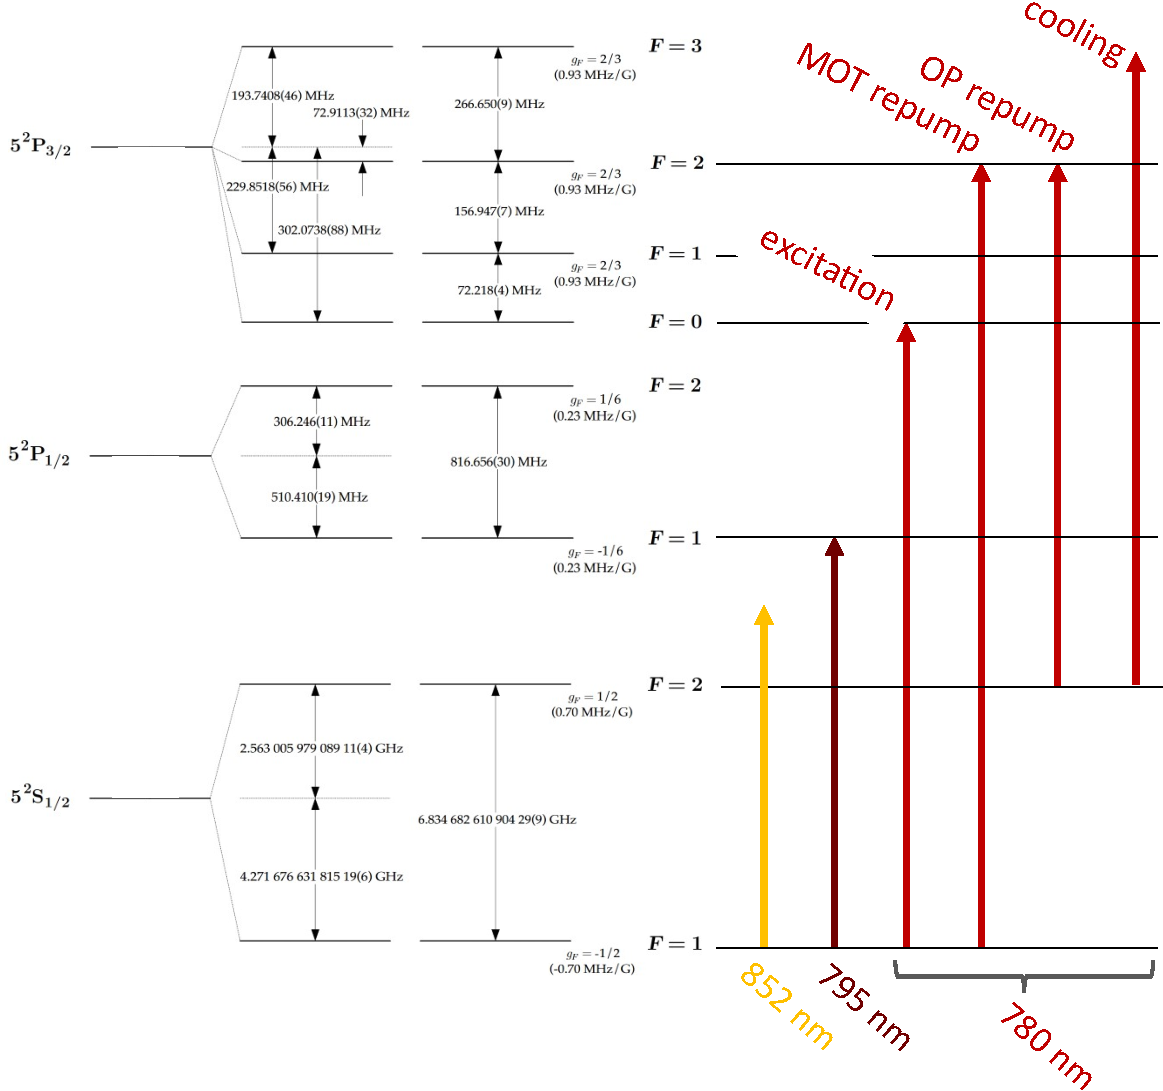
\includegraphics[width=0.9\textwidth]{Images/laser_frequencies.pdf}
    \caption{The different laser frequencies used in the quantum network experiment and their purposes.}
    \label{fig:laser_frequencies}
\end{figure}

\subsection{D2 Line cooling, excitation, and repumpers}

There are four laser frequencies with a nominal wavelength of 780 nm which we generate using only two distributed-feedback (DFB) laser sources (Eagleyard DFB Eagleyard EYP-DFB-0780-00080-1500-TOC03-0005) plus AOMs for frequency shifting. The two lasers supply two frequencies each, divided up by whether the relevant frequency is closer to resonance on the $D_2$ line with $F=1$ or $F=2$ in the ground state. In particular, one laser is locked on $F=1 \leftrightarrow F'=0$ and used to generate the excitation light (for generating single photons from the atoms) and the MOT repumper, while the other is locked on $F=2 \leftrightarrow F'=3$ and used for cooling/imaging and optical pumping (OP) repumper. Both lasers are locked using homebuilt saturated absorbtion setups in modulation transfer spectroscopy (MTS) configuration and homebuilt lockboxes.

The power of the individual DFB laser heads is insufficient for supplying power to both nodes, so each seeds a tapered amplifier (TA) for additional power. The cooling laser uses a homebuilt TA setup (with Eagleyard EYP-TPA-0780-03000-4006-CMT04-0000 TA chip) based on the design in \cite{kangara2014design}. The excitation laser seeds a commercially available fiber-coupled TA solution (MOGLabs MOAL with 785TA3000D TA chip) which provides over 1 W after the output fiber.

\begin{figure}[h!]
    \centering
    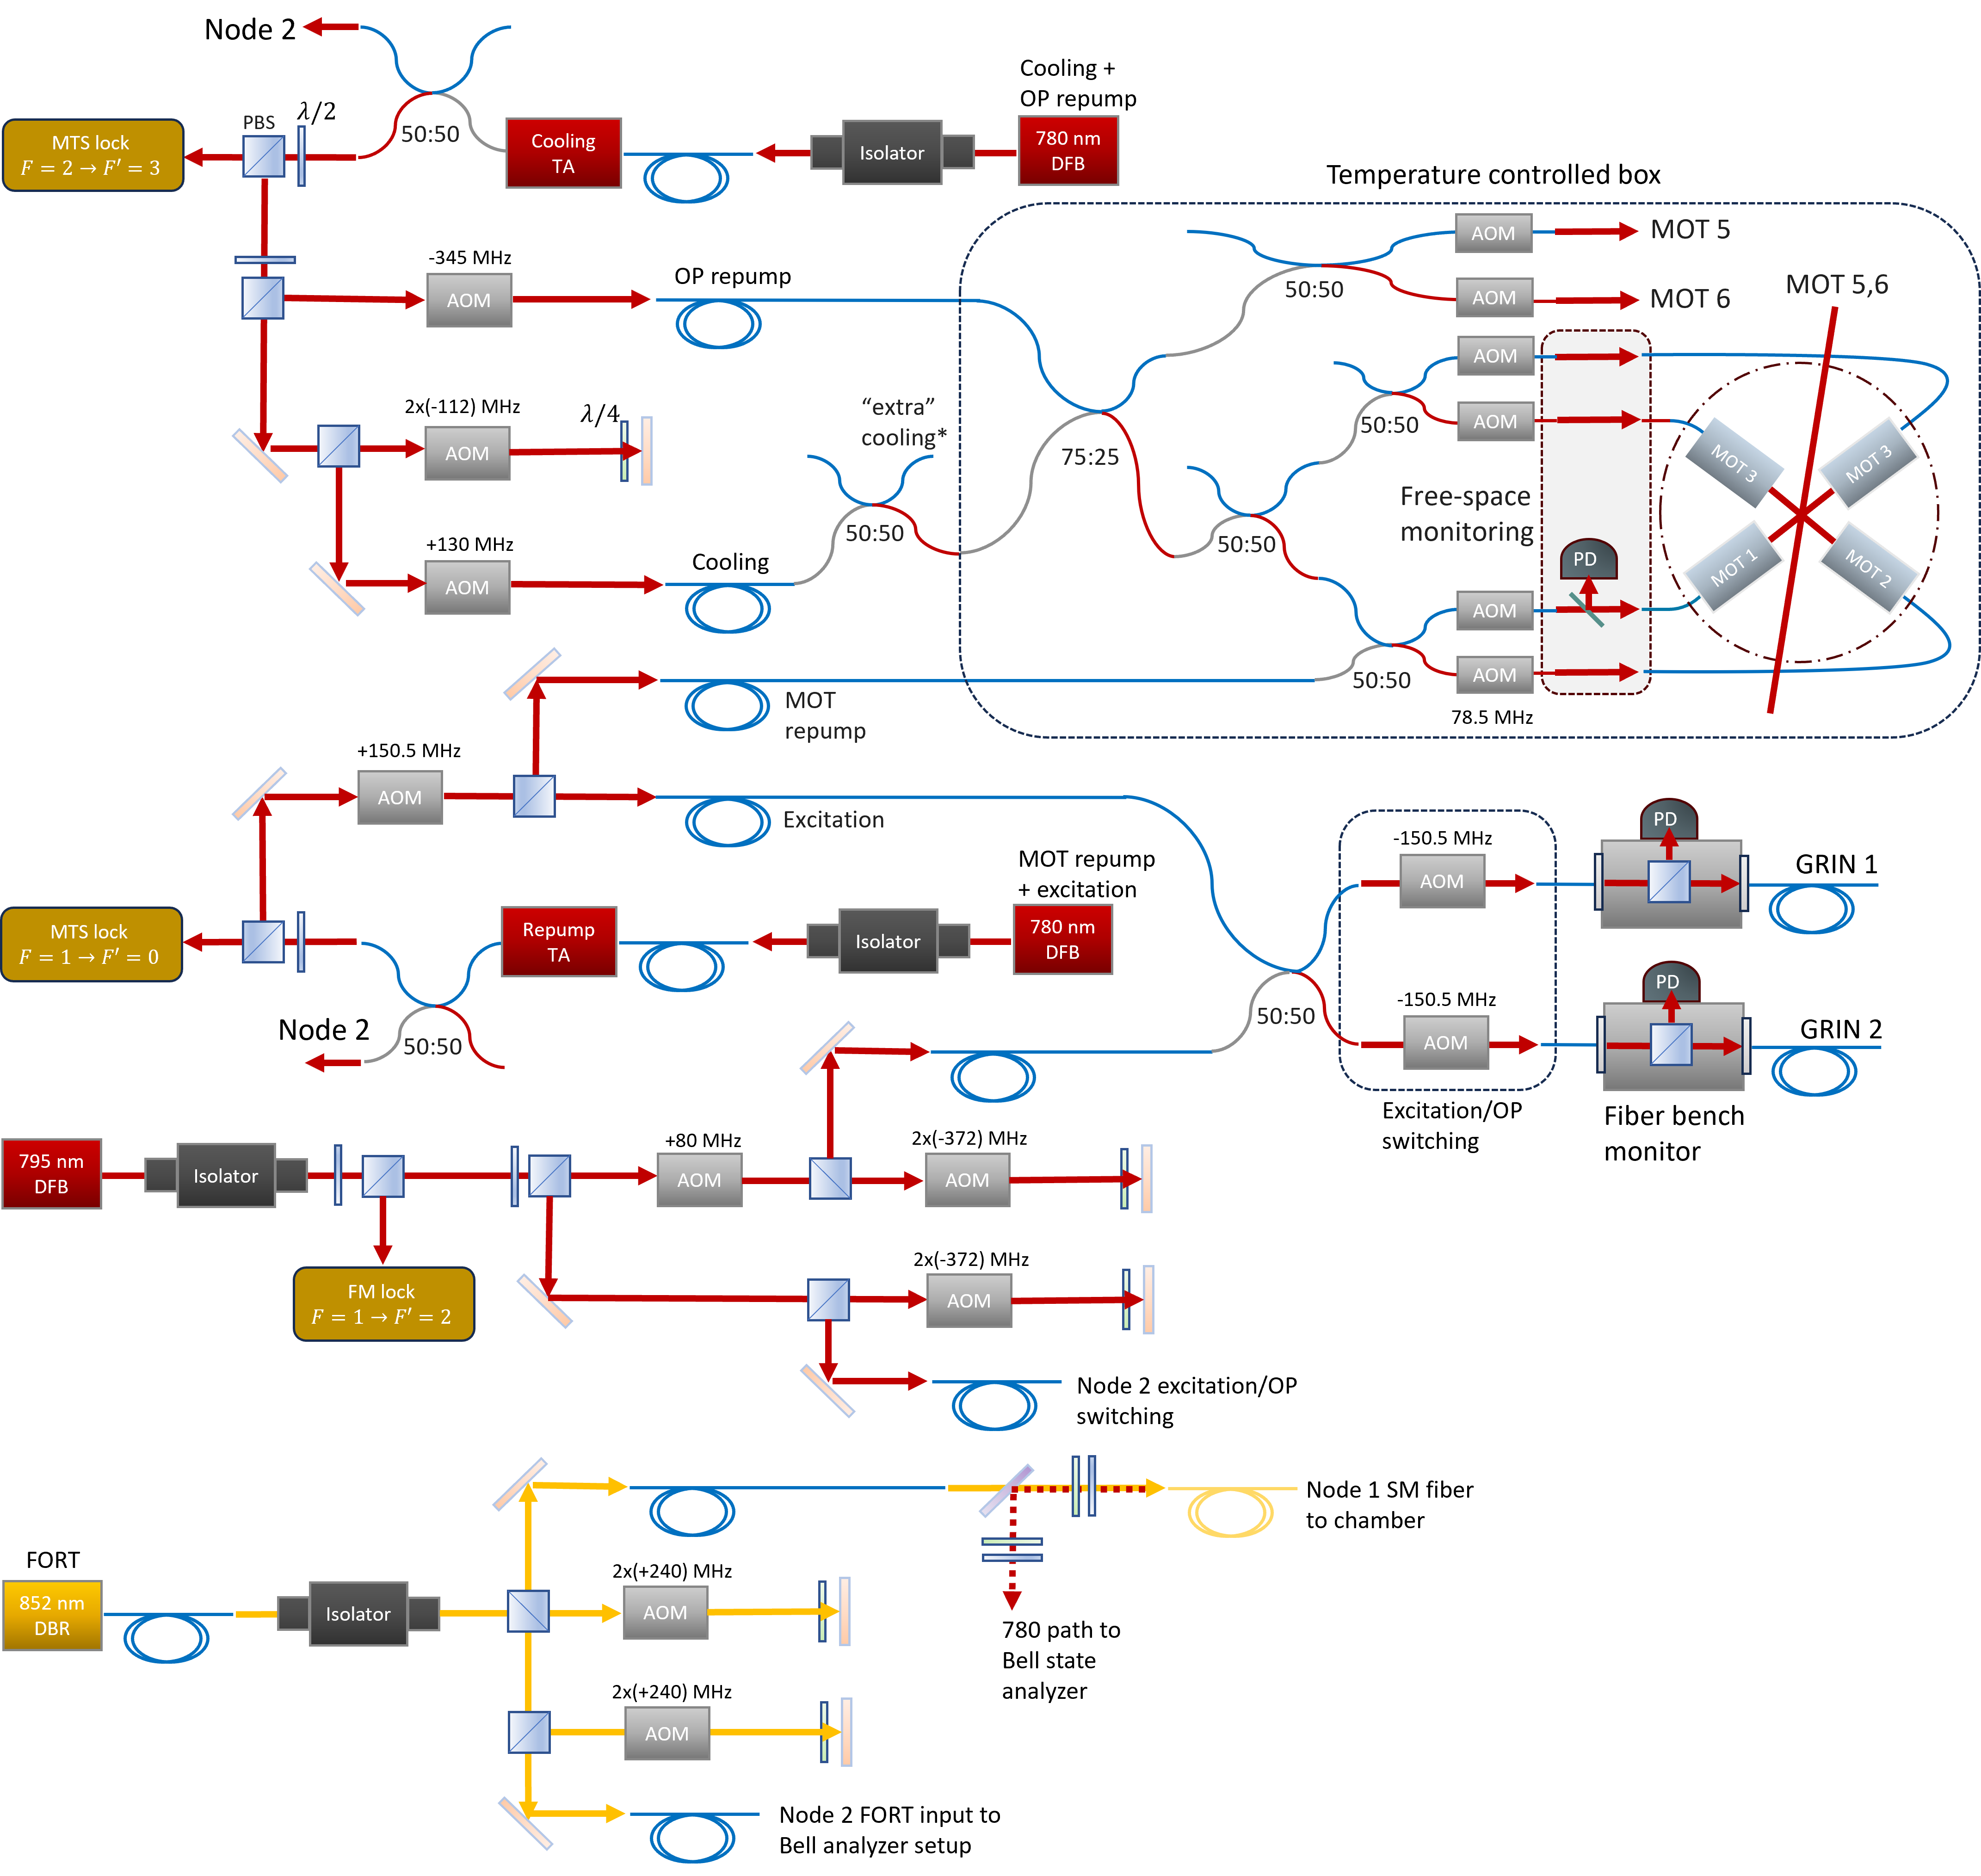
\includegraphics[width=0.9\textwidth]{Images/quantum_network_lasers_schematic.png}
    \caption{Schematic of the laser systems and routing for the quantum network experiment. Each laser head supplies both nodes, but only the common paths and those for one node (arbitrarily chosen to represent Node 1). The Node 2 setups are mostly duplicates of those for Node 1 except for some minor component-level differences.}
    \label{fig:all_lasers_schematic}
\end{figure}

The cooling, MOT repump, and OP repump are delivered to the science chamber's fibers through a fiber breakout made from PM fiber splitters (Thorlabs) linked with with PM butt connectors. Fiber-connectorized AOMs (CSRayzer AOM-780-78.5M-05-S-C1-PM780-1-1-1-FA) are used for introducing small frequency differences between MOT beams for standing wave mitigation, as well as switching of the MOT beam paths and performing dc intensity stabilization (see Sec. \ref{sec:fiber_AOM_power_stabilization}). 

\subsection{D1 Line optical pumping}

A 795 nm DFB laser (EYP-DFB-0795-00080-1500-TOC03-0005) resonant with $F=1 \leftrightarrow F'=1$ on the $D_1$ line is used for optically pumping the atoms into $\ket{F=1, m=0}$. This light shares a path to the atoms with the excitation light, where two AOMs are used for switching between two opposite directions (GRIN 1 and GRIN 2 paths in the chamber). This choice was made  because alternating between the two paths during optical pumping can reduce photo-scatter induced heating \cite{su2024fast}.

\subsection{FORT}
The dipole trap or far-off resonant trap (FORT), which we use interchangeably, is formed with a high-power 852 nm distributed Bragg reflector (DBR) laser (Photodigm 852.347DBRH-IBragg). The FORT light is coupled into the SM fiber interface to the science chamber after being combined with the 780 nm photon path using a dichroic beamsplitter (AVR Optics LPD02-785RU-25).  

\section{Magnetic field coils}
The coils for creating the quadrupole field for forming a MOT as well as shim fields and a bias field for entanglement experiments were made from Kapton-coated wire wrapped around custom aluminum holders designed by the author (Fig. \ref{fig:node1_coils.pdf}). The holders consist of six c-shaped sections, one for each coil which bolt to each other to form a frame which clamps to the chamber. The c-shape, rather than a closed loop, was chosen to mitigate the formation of eddy currents. The author notes that in retrospect, a non-metallic material or a variant of this design with fewer sharp edges would be preferable in a future build, as multiple shorts in the wires were found after wiring, apparently caused by the Kapton coating being worn off in certain places during the winding process. The version of coil holders used in the second node still suffered from this problem, despite design changes to reduce the number of edges encountered by the wires during winding.

\begin{figure}[h!]
    \centering
    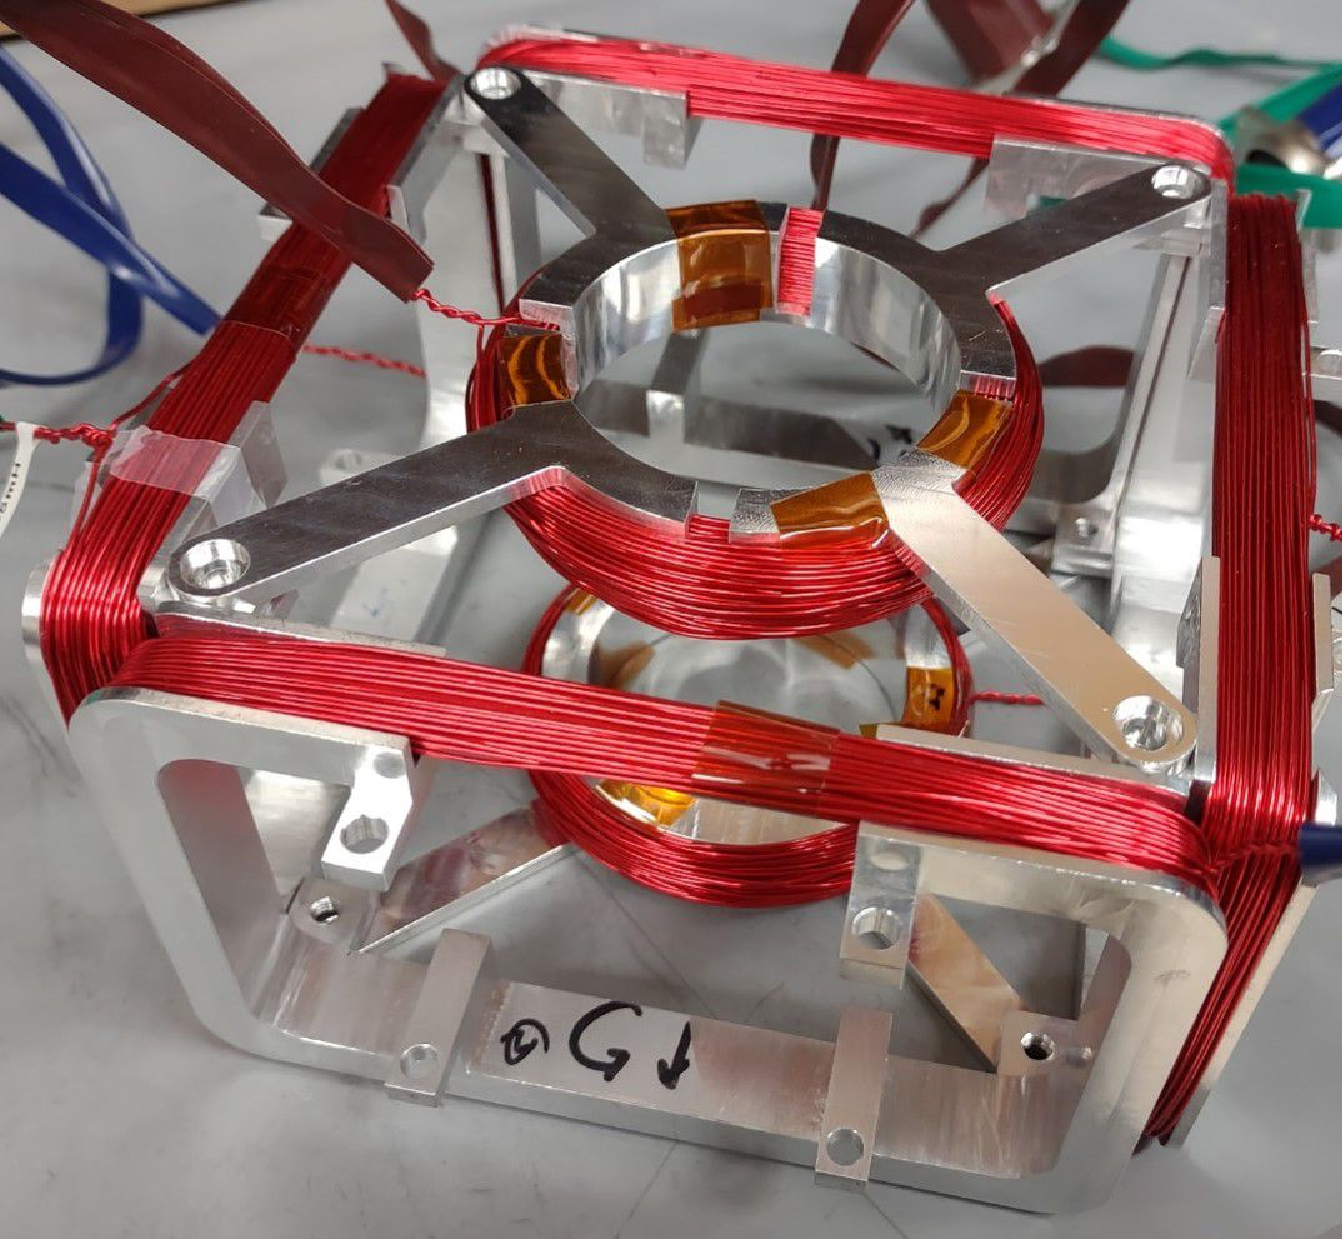
\includegraphics[width=0.7\textwidth]{Images/node1_coils.pdf}
    \caption{The coil assembly used for the first version of the quantum network experiment. A second version with minor modifications was made to give slightly deeper channels for the coils and notches to help start the winding. The circular coils can be driven in either an anti-Helmholtz or Helmholtz configuration to form a quadrupole field for the MOT or shim fields, respectively.}
    \label{fig:node1_coils.pdf}
\end{figure}

More details on preliminary coil testing will be given in the upcoming PhD thesis by Eunji Oh. Details on the design of the home-built coil drivers might be given in the upcoming PhD thesis by Jacob Scott. 

\section{MOT Geometry}

?? section needs fixing, particularly the equations. otherwise, omit entirely

The MOT geometry in the parabolic mirror version of the network node has no pairs of orthogonal beams among the three pairs, which is a result of the requirements imposed on the geometry by the in-vacuum optics and external objective lenses (see Fig. (\ref{fig:chamber_cross_section})). MOTs have been demonstrated with angles much less than 90 degrees between beam pairs (\cite{Garcia2013}), but the relative optical intensity in different pairs must be tuned to give comparable force gradients in each Cartesian direction.

\begin{figure}[h!]
    \centering
    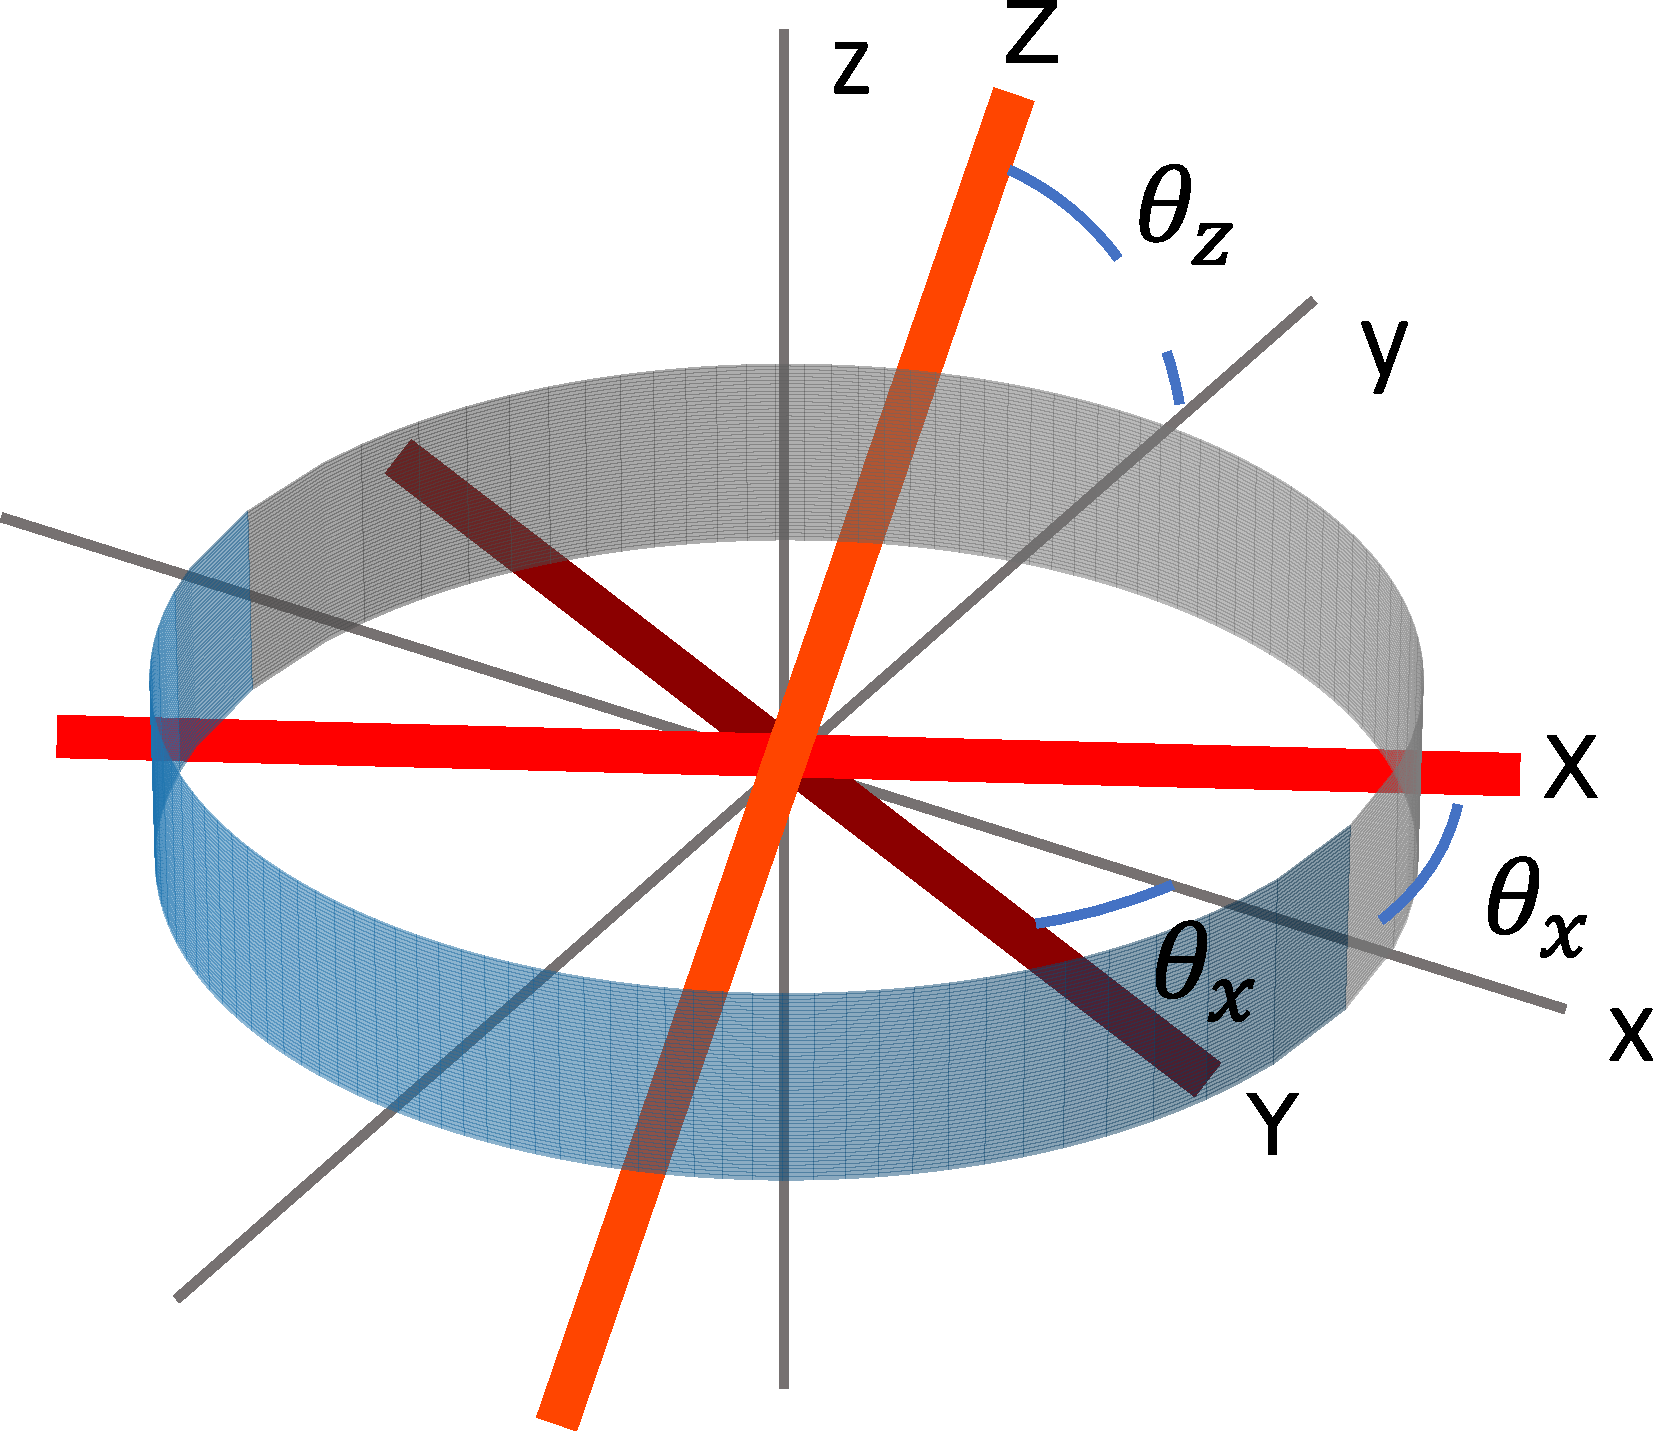
\includegraphics[width=0.5\textwidth]{Images/goofy_mot_beams.pdf}
    \caption{Non-orthogonal pairs of MOT beams. The cylindrical shell is intended to invoke a notion of where our vacuum chamber would be with respect to this set of beams. ?? double check this graphic}
    \label{fig:goofy_mot_beams}
\end{figure}

Consider a MOT with beam pairs X, Y, and Z, where X and Y lie in the $x-y$ plane and Z lies in the $y-z$ plane, with angles $\theta_x$ between the X/Y beams and the $x$ axis, and $\theta_z$ between Z and the $z$ axis, as in Fig. \ref{fig:goofy_mot_beams}. The two-level atom radiative force including the detuning of the light $\delta$ and Zeeman shift $\Delta_B$ due to a magnetic field due to a pair of beams $i$ is, in a low-intensity approximation, given by
\begin{equation}
    F_i(\mathbf{r}) = \frac{s_i}{1 + s_i + 4(\delta + \Delta_B(\mathbf{r}) \hat{B}(\mathbf{r})\cdot\hat{e}_i)^2/\gamma^2} - \frac{s_i}{1 + s_i + 4(\delta - \Delta_B(\mathbf{r}) \hat{B}(\mathbf{r})\cdot\hat{e}_i)^2/\gamma^2}
\end{equation}\label{eq:force_i}
where $\hat{B}\cdot\hat{e}_i$ gives the dot product of the magnetic field at a particular point in space with the propagation axis of the beams and $s_i$ is the saturation parameter, assumed to be equal for both beams in the pair. For the beams denoted X,Y, and Z as defined, the forces along Cartesian directions $\hat{x},\hat{y}$ and $\hat{z}$ are
\begin{align}
    F_x &= F_X \cos{\theta_x} + F_Y \cos{\theta_x} \\
    F_y &= F_X \sin{\theta_x} + F_Y \sin{\theta_x} + F_Y \sin{\theta_z} \\
    F_x &= F_Z \cos{\theta_z}
\end{align}
where the $F_i$ on the RHS are given by Eq. (\ref{eq:force_i}). In order to find beam intensities which give a symmetric MOT in $\hat{x}$ and $\hat{y}$, we can find solve the system 
\begin{align}
    \nabla F_y &= \nabla F_x \\
    \nabla F_x &= -\kappa \nabla F_z \\
    s_x &= s_y
\end{align}
for $s_y, s_z$, and $\kappa$, evaluated at $x=y=z=0$, where $\kappa$ is a positive-valued constant. We can approximate the magnetic quadrupole field by $B = B_0 (-x/2 \hat{x} -y/2 \hat{y} + z\hat{z})$

% If the radiative force including the spatially-dependent Zeeman shifts along the $i^{\textrm th}$ beam pair is $f_i$, we can compute the forces $F_{i}$ along each Cartesian axis $i$: ?? not correct

% \begin{align}
%     F_x = f_x \cos(\theta_x) + f_y \cos(\theta_x) \nonumber \\
%     F_y = f_x \sin(\theta_x) + f_y \sin(\theta_x) + f_z \sin(\theta_z) \\
%     F_z = f_z \cos(\theta_z) \nonumber
% \end{align}

\section{Experiment Control}

Quantum networking experiments with cold atoms require control hardware including analog and digital inputs and outputs, each with a high degree of timing precision. It is also important to be able to write flexible control programs which streamline experiment runs, including data acquisition and analysis. For these purposes, we use the Sinara hardware suite and ARTIQ control software. Our Sinara hardware consists of analog and digital I/O and DDS channels controlled by a Zynq-based FPGA controller, the Kasli-SoC\cite{lam2021combining}. The benefit of FPGA-controlled hardware, as opposed to looping a predetermined pulse sequence, is the ability to have experiments with conditional logic which determines how the experiment progresses. This is particularly important for the probabilistic entanglement sequence described in Sec. \ref{sec:reg}, in which a detection event heralding remote entanglement can be used to break out of the entanglement attempt loop to use the entanglement as a resource. Breaking out of the loop is also a necessity for verifying the state with quantum state tomography and for reloading atoms when one is lost.

For one-node operation described in this thesis, each network node is independently controlled by its own Sinara hardware and ARTIQ instance. However, for two-node operation, the FPGA controllers (Kasli-SoC) can be operated in a satellite configuration in which one operates as a master while the other(s) follows and the two share a clock \cite{Stephenson2020}. 

% could make a figure showing how many channels are controlling each thing?